\documentclass{article}

\usepackage[a4paper,top=3cm,bottom=3cm,left=3cm,right=3cm,marginparwidth=1.75cm]{geometry}

% Useful packages
\usepackage{amsmath}
\usepackage{graphicx}
\usepackage{blindtext}
\usepackage{tabularx}
\usepackage{enumitem}
\usepackage{longtable}
\usepackage{array,booktabs,enumitem}
\usepackage{titlepic}
\usepackage[colorlinks=true, allcolors=blue]{hyperref}
\usepackage[nameinlink]{cleveref}
\usepackage[backend=biber, style=authoryear, sorting=ynt, maxnames=1]{biblatex}
\usepackage{titling}
\usepackage{subcaption}
\addbibresource{ref.bib}


\newcommand{\subtitle}[1]{%
  \posttitle{%
    \par\end{center}
    \begin{center}\LARGE#1\end{center}
    \vskip0.3em}%
}

\makeatletter
\newcommand*{\linkblx@startlink}[1]{%
  \blx@sfsave\hyper@natlinkstart{\the\c@refsection @#1}\blx@sfrest}
\newcommand*{\linkblx@startlinkentry}{%
  \linkblx@startlink{\abx@field@entrykey}}
\newcommand*{\linkblx@endlink}{%
  \blx@sfsave\hyper@natlinkend\blx@sfrest}

\DeclareCiteCommand{\cite}
  {}%
  {\DeclareFieldFormat{bibhyperref}{####1}%
   \linkblx@startlinkentry
   \ifnumequal{\value{citecount}}{1}
     {\usebibmacro{prenote}}
     {}%
   \usebibmacro{citeindex}%
   \usebibmacro{cite}%
   \ifnumequal{\value{citecount}}{\value{citetotal}}
     {\usebibmacro{postnote}}
     {}%
   \iflastcitekey{}{\multicitedelim}%
   \linkblx@endlink}
  {}
  {}

\DeclareCiteCommand*{\cite}
  {}%
  {\DeclareFieldFormat{bibhyperref}{####1}%
   \linkblx@startlinkentry
   \ifnumequal{\value{citecount}}{1}
     {\usebibmacro{prenote}}
     {}%
   \usebibmacro{citeindex}%
   \usebibmacro{citeyear}%
   \ifnumequal{\value{citecount}}{\value{citetotal}}
     {\usebibmacro{postnote}}
     {}%
   \iflastcitekey{}{\multicitedelim}%
   \linkblx@endlink}
  {}
  {}

\DeclareCiteCommand{\parencite}
  {}%
  {\DeclareFieldFormat{bibhyperref}{####1}%
   \linkblx@startlinkentry
   \iffirstcitekey{\bibopenparen}{}%
   \ifnumequal{\value{citecount}}{1}
     {\usebibmacro{prenote}}
     {}%
   \usebibmacro{citeindex}%
   \usebibmacro{cite}%
   \ifnumequal{\value{citecount}}{\value{citetotal}}
     {\usebibmacro{postnote}}
     {}%
   \iflastcitekey{\bibcloseparen}{\multicitedelim}%
   \linkblx@endlink}
  {}
  {}

\DeclareCiteCommand*{\parencite}
  {}%
  {\DeclareFieldFormat{bibhyperref}{####1}%
   \linkblx@startlinkentry
   \iffirstcitekey{\bibopenparen}{}%
   \ifnumequal{\value{citecount}}{1}
     {\usebibmacro{prenote}}
     {}%
   \usebibmacro{citeindex}%
   \usebibmacro{citeyear}%
   \ifnumequal{\value{citecount}}{\value{citetotal}}
     {\usebibmacro{postnote}}
     {}%
   \iflastcitekey{\bibcloseparen}{\multicitedelim}%
   \linkblx@endlink}
  {}
  {}


\DeclareCiteCommand{\textcite}
  {\boolfalse{cbx:parens}}
  {\DeclareFieldFormat{bibhyperref}{####1}%
   \linkblx@startlinkentry
   \usebibmacro{citeindex}%
   \iffirstcitekey
     {\setcounter{textcitetotal}{1}}
     {\stepcounter{textcitetotal}%
      \textcitedelim}%
   \usebibmacro{textcite}%
   \iflastcitekey
     {}
     {\ifbool{cbx:parens}
        {\bibcloseparen\global\boolfalse{cbx:parens}}
        {}}%
   \ifnumequal{\value{citecount}}{\value{citetotal}}
     {\usebibmacro{textcite:postnote}}
     {}%
   \linkblx@endlink}
  {}
  {}

\DeclareMultiCiteCommand{\parencites}{\parencite}{}
\makeatother

\subtitle{Group 9 - Machine Visual Perception Project Report}
\title{
    \begin{center}
    
\includegraphics[width=0.45\textwidth]{cst.jpg}~
    \\[0.1cm]
    \Huge Auto-Initialising Differentiable Renderers
    \end{center}
}
\author{Pranav Talluri, Ke Ding, Yujia Yang}
\date{2022}

\begin{document}


\maketitle
\newpage
\tableofcontents
\newpage
\section{Introduction and Motivation}
\subsection{Introduction to the Problem}

Rendering allows us to produce 2D images from 3D scene data. A common problem in computer vision is inverse rendering, which is the process of estimating physical attributes of a scene (3D) from an image (2D).

Traditional approaches to constructing 3D scenes are typically based on carefully controlled, high quality capture of the scene using specialised equipment and algorithms to construct the scene based on the captured data. 

Deep learning approaches learn a mapping between images and scenes. These approaches require very large amounts of data and are not very generalisable.
Inverse rendering approaches aim to infer the scene that an image (or set of images) is based on by rendering scenes, comparing the images and the renders and backpropagating changes to improve the loss between them. The key requirement for inverse rendering is for the rendering operation to be differentiable for the backpropagation to be possible. However, in order to construct an image of visible objects from a scene, most rendering pipelines utilise rasterisation, which is not differentiable.

Inverse rendering utilises differentiable renderers to circumvent the rasterisation stage of typical rendering pipelines. Differentiability means we can backpropagate changes, so that searching for an optimal scene estimate is as simple as performing stochastic gradient descent over the scene parameters. We focus on SoftRas \parencite{softras}, a rendering pipeline that introduces soft rasterisation, an alternative method of determining the visibility of elements in the scene.

Soft rasterisation utilises a probabilistic interpretation of visibility to maintain the differentiability of the rendering pipeline. Specifically, it identifies the probability of mesh triangles contributing to pixels, rather than the traditional (undifferentiable) discrete sampling approach. The probabilities are aggregated using depth information and colour maps to determine the pixel values of the image.

SoftRas allows us to perform image-based shape deformation. This is where we reconstruct the mesh of an object by providing multiple images of the object from various viewpoints. Specifically, we provide a set of silhouettes of an object, their viewpoints and an initial mesh and SoftRas will attempt to fit the mesh according to the silhouettes.

The key problem we try to address in this project is the initialisation of SoftRas, and the insights we develop will be applicable to differentiable renderers in general. The search space for determining the optimal mesh is large and high-dimensional, so the initialisation can have a significant impact on the quality of the fitted mesh, the amount of iterations required and whether SoftRas is able to converge at all or becomes stuck in local minima.

\newpage
\subsection{Background and Related Work}

The key literature for this project is \emph{Soft Rasterizer: A Differentiable Renderer for Image-based 3D Reasoning} \parencite{softras}. The paper introduces a novel approach to differentiable rendering, replacing the standard discrete rasterisation process with a new soft rasteriser as discussed in \ref{section:softraspipealgo}. We specifically investigate the usage of the differentiable renderer to perform inverse rendering. Figure \ref{softrasresults} shows the fitting procedure, which is discussed further in \ref{section:softrasalgo}.

\begin{figure}[h!]
  \centering
  \begin{subfigure}{0.45\textwidth}
    \centering
    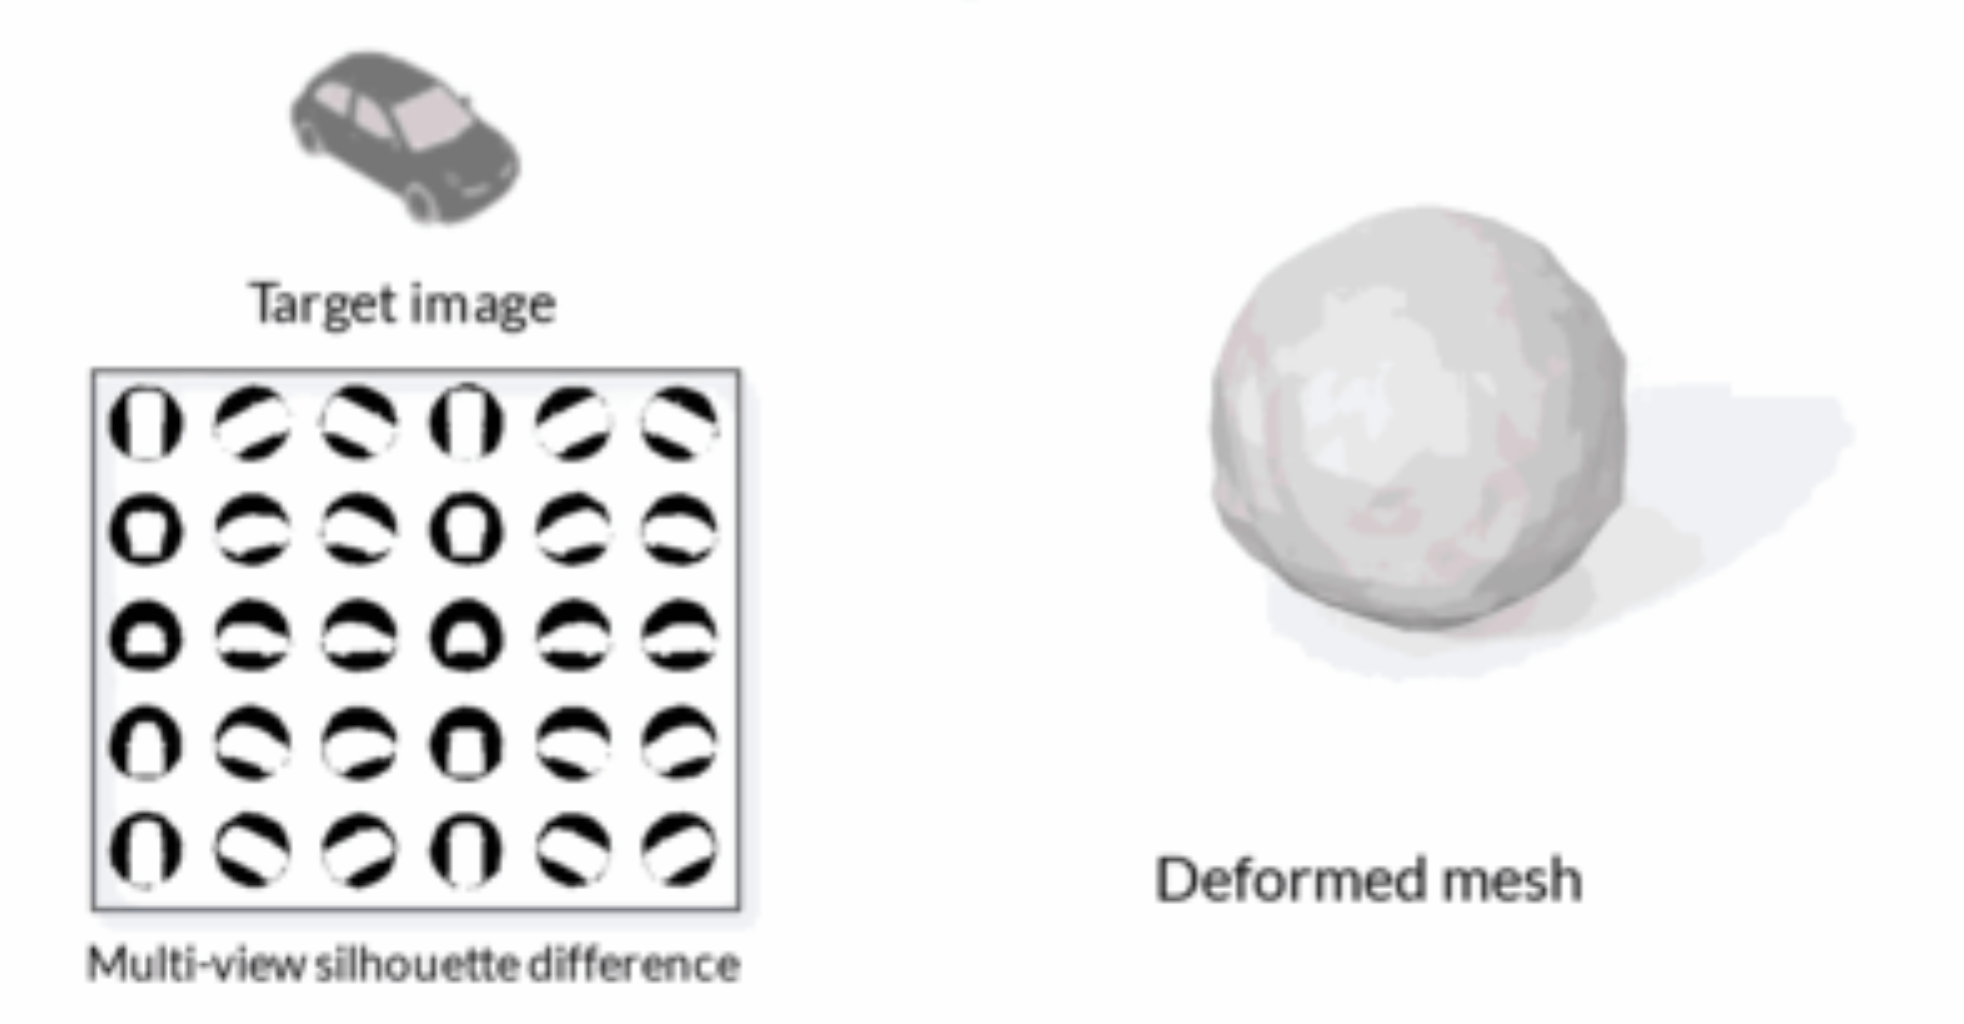
\includegraphics[width=\textwidth]{images/softrasinit.png}
    \caption{Start}
    \label{softrasstart}
  \end{subfigure}
  \hfill
  \begin{subfigure}{0.45\textwidth}
    \centering
    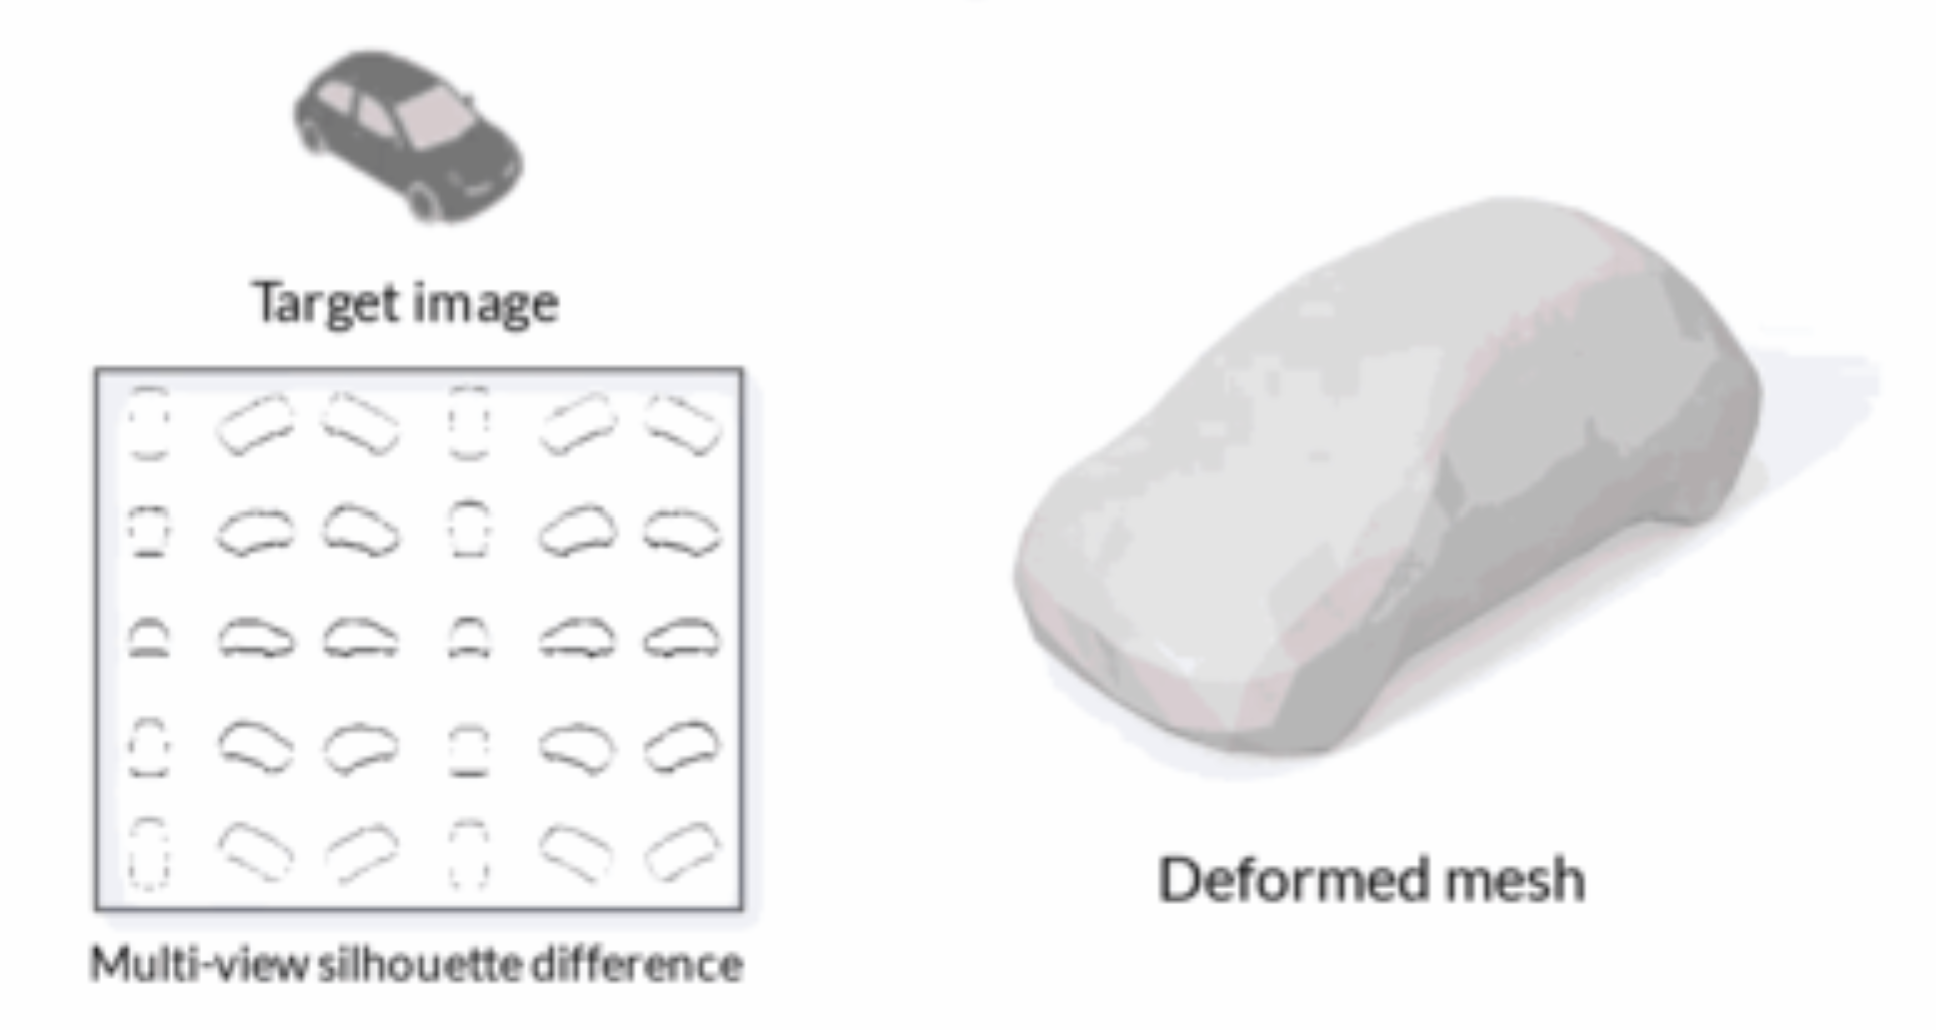
\includegraphics[width=\textwidth]{images/softrasresults.png}
    \caption{End}
    \label{softrasend}
  \end{subfigure}
  \caption{SoftRas fitting procedure}
  \label{softrasresults}
\end{figure}

Our project also uses on DeepLabv3 \parencite{deeplab} for generating image silhouettes. DeepLabv3 utilises modules which employ atrous convolution in cascade or parallel to capture multi-scale context by adopting multiple atrous rates. Atrous convolution enables adding more layers (deeper networks) without having to have larger images, as shown in Figure \ref{deeplabatrousnoatrous}. It utilises pyramid pooling modules to probe convolutional features at multiple scales.

\begin{figure}[h!]
  \centering
  \begin{subfigure}{\textwidth}
    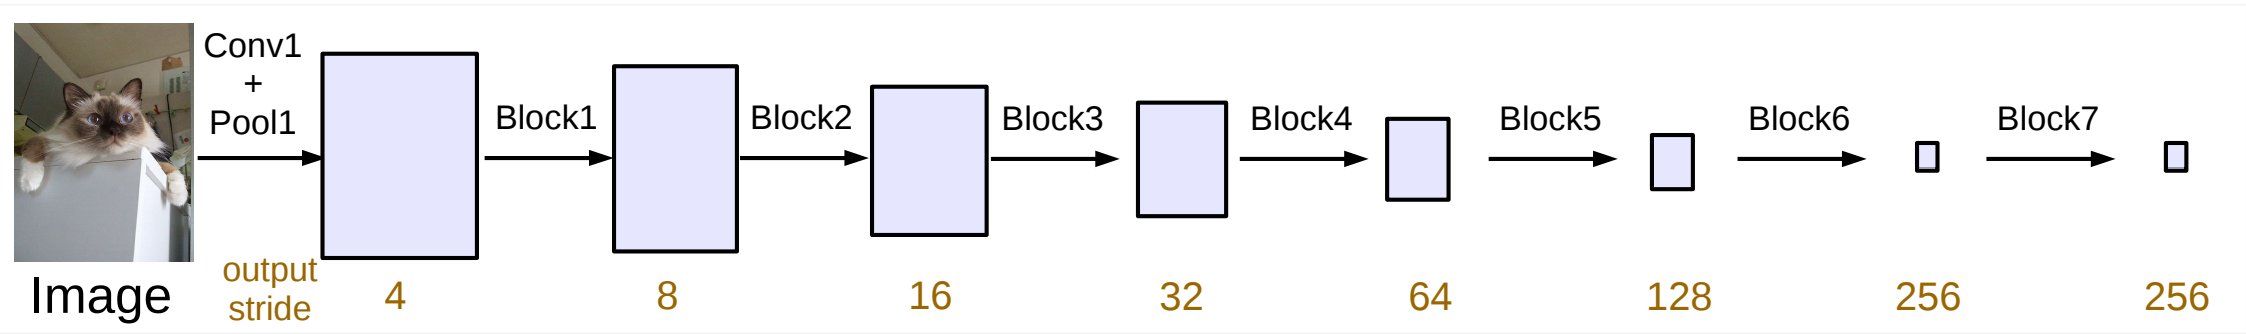
\includegraphics[width=\textwidth]{images/deeplabnoatrous.png}
    \caption{Without atrous convolutions}
    \label{deeplabnoatrous}
  \end{subfigure}
  \begin{subfigure}{\textwidth}
    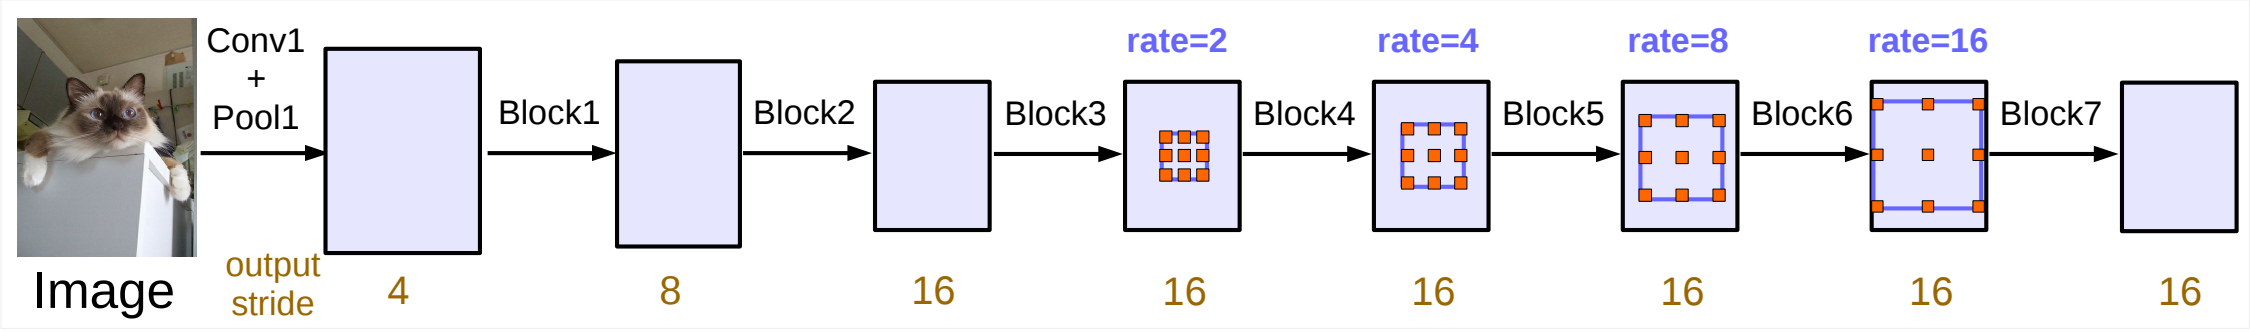
\includegraphics[width=\textwidth]{images/deeplabatrous.png}
    \caption{With atrous convolutions}
    \label{deeplabatrous}
  \end{subfigure}
  \caption{Cascaded modules with \ref{deeplabatrous} and without \ref{deeplabnoatrous} atrous convolution}
  \label{deeplabatrousnoatrous}
\end{figure}

DeepLab is able to generalise well to new images due to its large and varied training dataset. The authors of the original paper also detail the typical failure modes. The model is able to perform extremely well on images with clear subjects but is weaker when given images without a clear view of the subject or differentiating between similar subject classes. The latter failure mode is not a concern for our usage of DeepLab. Some sample results are shown in Figure \ref{deeplabresults} where the first two rows show successful results and the last row visualises the failure modes.

\begin{figure}[h!]
  \centering
  \begin{subfigure}{\textwidth}
    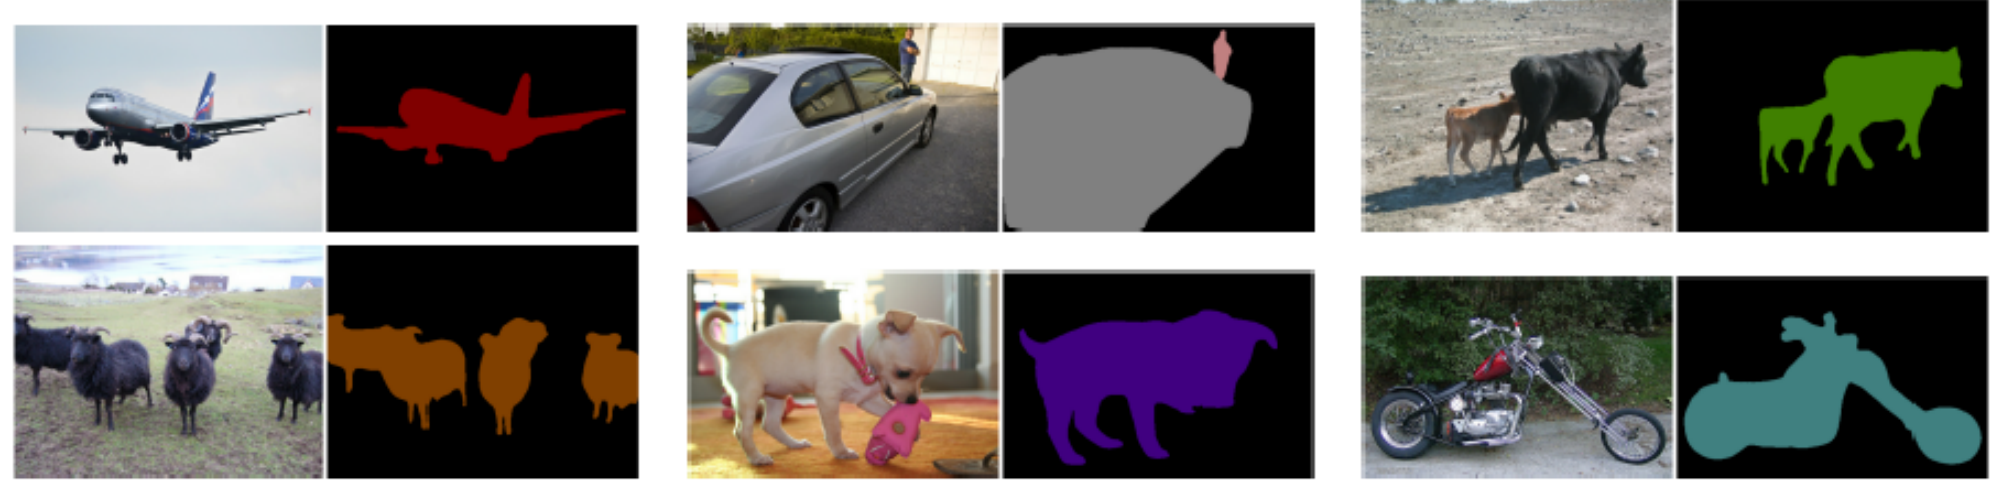
\includegraphics[width=\textwidth]{images/deeplabresultsgood.png}
    \caption{Good results}
    \label{deeplabresultsgood}
  \end{subfigure}
  \begin{subfigure}{\textwidth}
    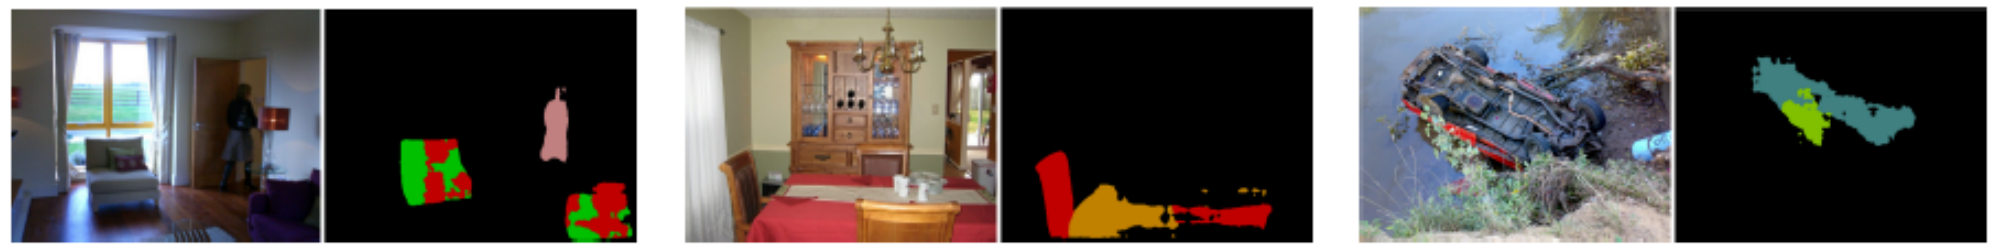
\includegraphics[width=\textwidth]{images/deeplabresultsbad.png}
    \caption{Failure modes}
    \label{deeplabresultsbad}
  \end{subfigure}
  \caption{Samples from the original paper, including failure modes}
  \label{deeplabresults}
\end{figure}

\subsection{Overview of the Idea}

The aim of our project is to address the initialisation of SoftRas, in order to improve its performance in constructing a fitted mesh when given images of an object from multiple viewpoints. There are three key initialisations for SoftRas which we aim to address: silhouettes, meshes and camera parameters. In addition to these initialisations, we also investigate the data used. The original paper uses a subset of the ShapeNet \parencite{shapenet} dataset, which features renders of artificial 3D models of simple objects that fit into a small number of classes.

\subsubsection{Silhouette Initialisation}

The first initialisation is the silhouettes of the multi-view images. The original softras pipeline directly takes silhouettes of the object to be reconstructed. This is possible because the authors construct renders from the ShapeNet dataset which already have a transparent background. This is problematic as most real world multi-view datasets feature full images, including a background. To address this problem, we will utilise semantic segmentation (DeepLab) to produce segmentation masks, which can then be used to generate silhouettes. Retrofitting this pipeline to SoftRas will enable us to reconstruct objects from natural images.

\subsubsection{Mesh Initialisation}

The next initialisation is the mesh that SoftRas deforms to fit to the input images. By default, the SoftRas pipeline utilises a sphere. The initial mesh has a large impact on the both the number of iterations required by the fitting procedure and the final product. We plan on modifying this initialisation based on the input images to accelerate the fitting procedure and procedure better results. The modifications are: manipulating the polygon count of the mesh, changing the scale of the sphere and translating its position.

\subsubsection{Dataset Investigation}

The data used in the original paper comes from the ShapeNet dataset. This has some key limitations. The images utilised are relatively low resolution (64x64) and are not natural images, they come from renders of computer generated 3D models. In our project, we aim to investigate the effectiveness of SoftRas on higher resolution, photorealistic images. We achieve this primarily by experimenting with the Amsterdam Library of Object Images (ALOI) \parencite{aloi} dataset, which contains photographic images of a large variety of objects with resolutions of 384x288. The images are also taken from more limited viewpoints (no vertical viewpoint variation), which will test the fitting procedure's ability to extend to less informative input images. This dataset includes the ground truth camera parameters, so we also aim to test the pipeline on images that we capture ourselves where the ground truth for image viewpoints is not known and the backgrounds are more challenging.

\subsubsection{(Extension) Camera Parameter Initialisation}

The final initialisation is the viewpoint labels for each of the multi-view silhouettes passed as input to the fitting procedure. These parameters tell the fitting procedure which angles to generate renders of the predicted mesh from so that these renders can be compared to the silhouettes to compute a loss. The fitting procedure used in the original paper utilises ground truth viewpoint labels that are given by the ShapeNet dataset. We aim to estimate these parameters using SfM in order to enable fitting on natural images where the ground truth viewpoint parameters are unknown.

\newpage
\section{Method}
\subsection{Baseline Algorithm}
\subsubsection{Soft Rasteriser}
\label{section:softraspipealgo}

The backbone of our project is the official implementation of SoftRas created by the authors of the paper. We utilise the soft rasteriser from this original project in order to generate renders of the predicted model. Figure \ref{softraspipe} compares the rendering pipeline used by SotfRas and a traditional pipeline.

\begin{figure}[h!]
  \centering
  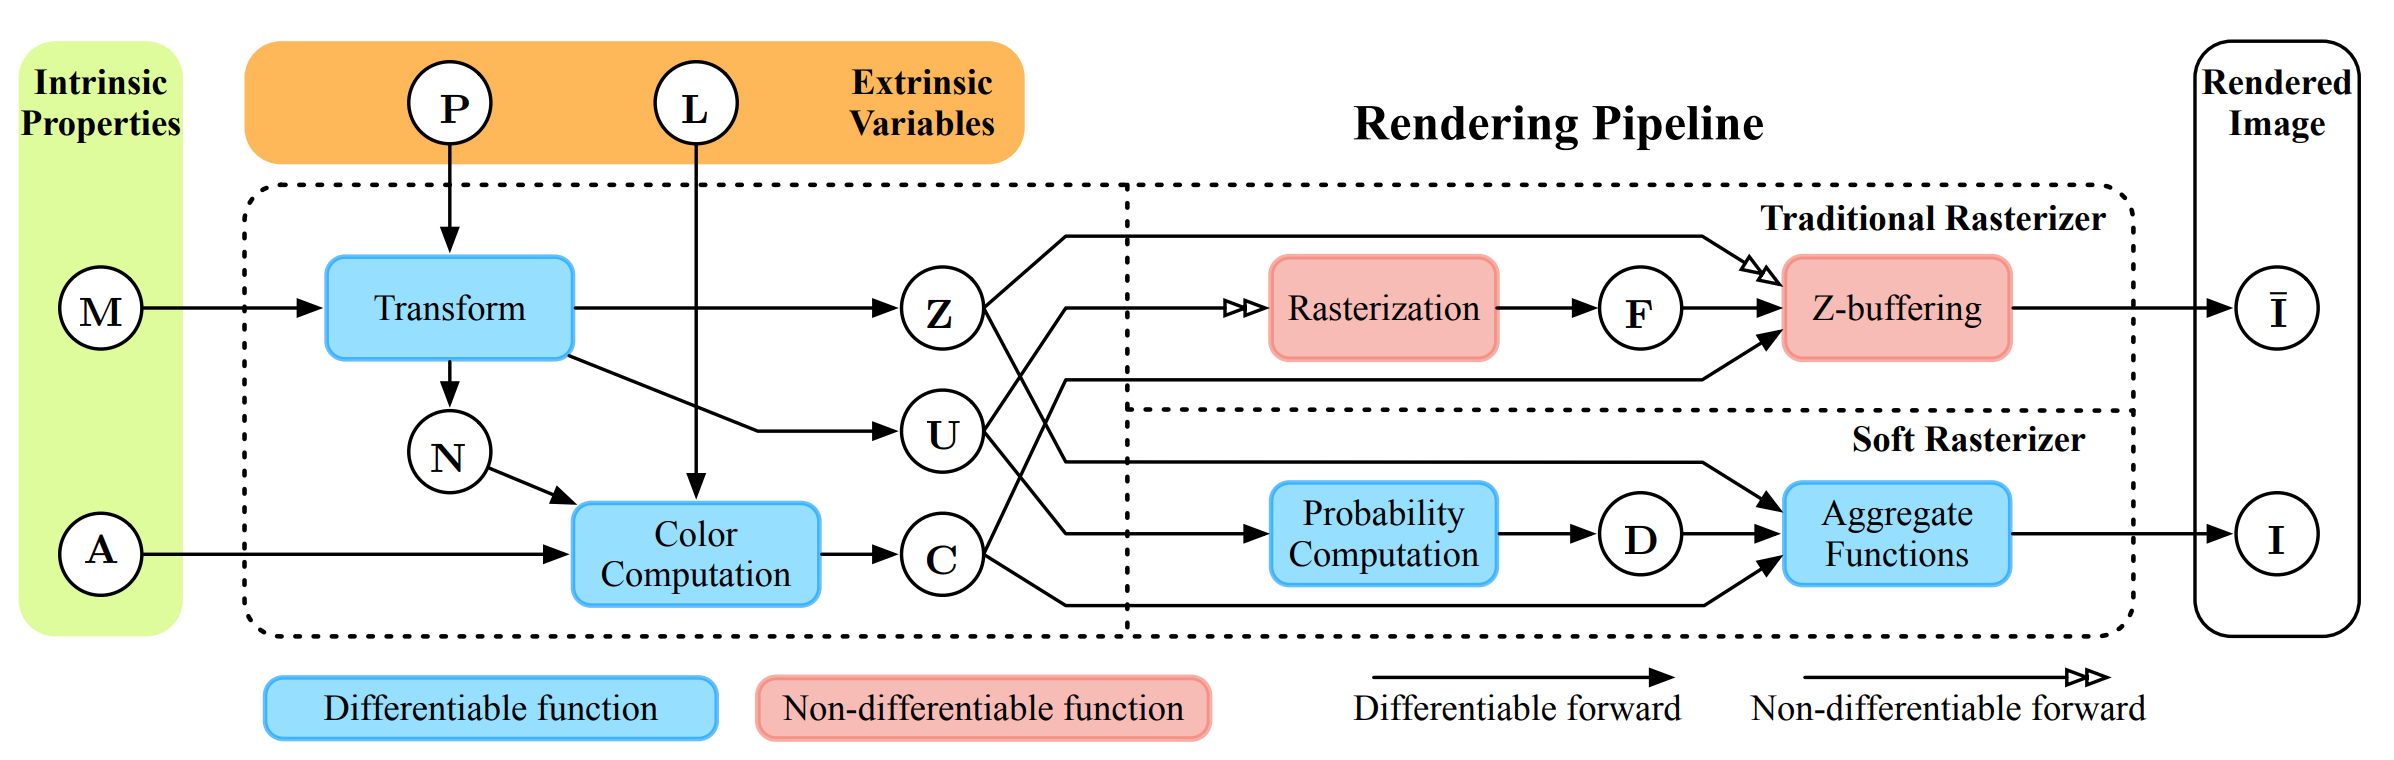
\includegraphics[width=\textwidth]{images/softraspipeline.png}
  \caption{SoftRas vs Traditional Rendering Pipeline}
  \label{softraspipe}
\end{figure}

The soft rasteriser works by aggregating probabilistic contributions from each triangle in the scene mesh, which makes it truly differentiable. This is a notable improvement over prior works in differentiable renderers, which only approximate the rendering gradient in the back propagation stage, and utilise traditional methods in the forward pass, such as \cite{neural3dmeshrenderer}. SoftRas therefore avoids an inconsistency between the forward and backward passes which would lead to uncontrolled optimisation behaviours and a limited ability to generalise to other 3D reasoning tasks.

SoftRas interprets rasterisation as a problem of binary masking determined by the relative positions between pixels and triangles, and z-buffering merges rasterisation results on a per-pixel basis using the relative depths of triangles. SoftRas then aims to solve this problem in a differentiable manner, which it achieves utilising probability maps $\{D_j\}$ and an aggregation function $A$. $D_j$ models the influence of triangle mesh $f_j$ on the image plane. We need to estimate this value using a function, which needs to take into account the relative position and distance between the pixel $p_i$ and triangle $f_j$. We define $D_j^i$ using the sigmoid function \[D^i_j = sigmoid(\delta^i_j \times \frac{d^2(i,j)}{\sigma})\text{.}\]

For each mesh triangle $f_j$, we define its colour map $\{C_j\}$ at pixel $p_i$ on the image plane by interpolating vertex colour using barycentric coordinates.

$A$ is an aggregate function that we use to merge the colour maps $\{C_j\}$ and obtain rendering output $I$ based on probability maps $\{D_j\}$ and the relative depths $\{z_j\}$. Figure \ref{softrasraster} shows how this compares with a traditional, discrete rasterisation pipeline.

\begin{figure}[h!]
  \centering
  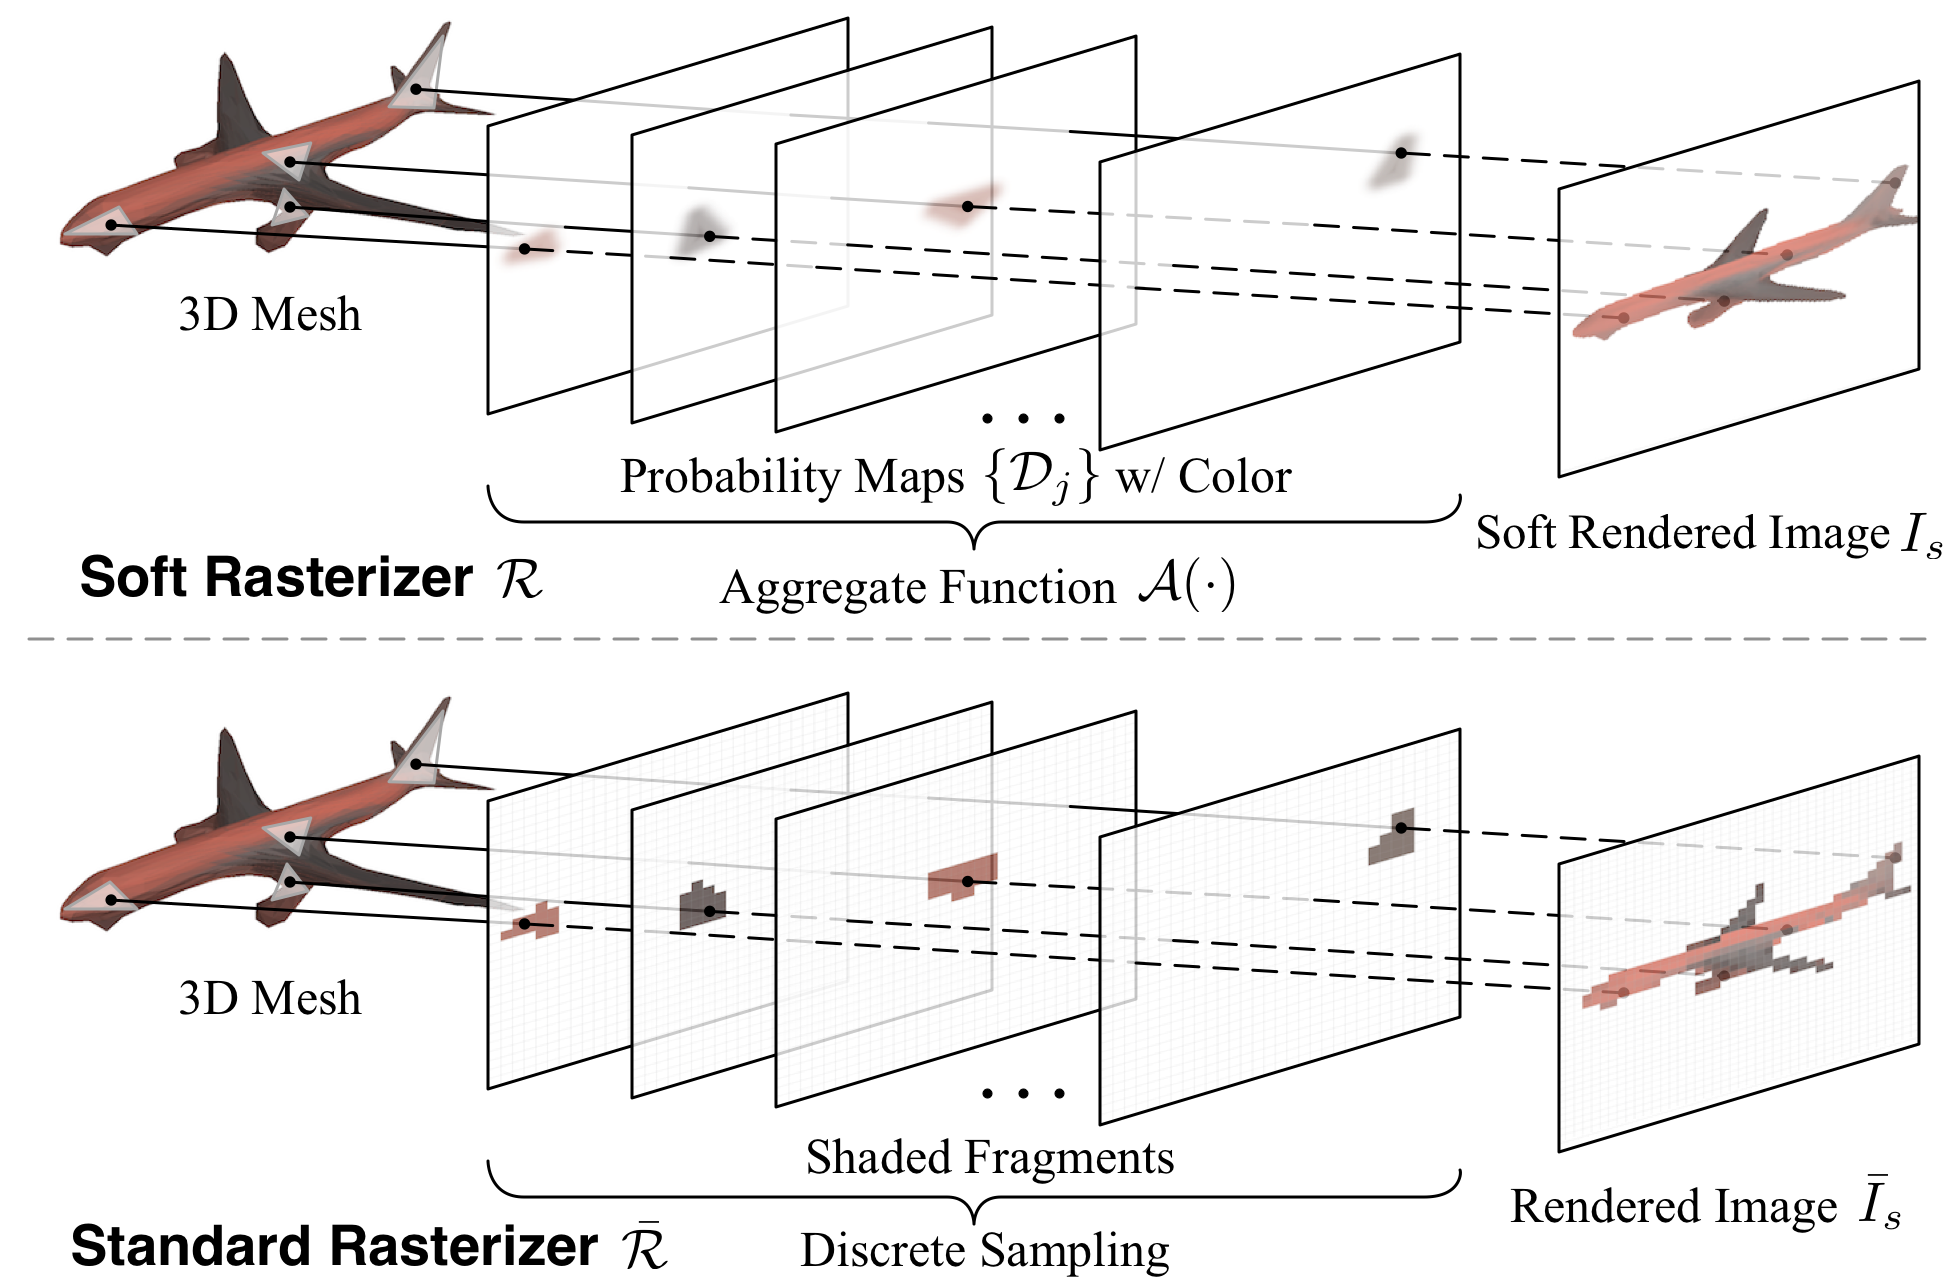
\includegraphics[width=0.7\textwidth]{images/softras.png}
  \caption{SoftRas vs Traditional Rasteriser}
  \label{softrasraster}
\end{figure}

\subsubsection{Fitting Procedure}
\label{section:softrasalgo}
Given an initial mesh, the procedure makes changes to the faces and vertices of the mesh, produces 2D renders of this mesh using the soft rasteriser and then compares these renders to the input images to compute a loss. This loss is then used to inform backpropagation through the rendering pipeline to modify the mesh. In fact, the original procedure takes pairs of viewpoints for every batch to compute a single loss. This repeats for some large number of iterations. The initial mesh, therefore, has a large impact on the performance of the process, including the number of iterations required to converge, the mesh that is converged at and whether or not the procedure is able to converge.

The loss is computed using the intersection over union (IoU). This is a common loss used when fitting shapes. Given a set of $n$ ground truth images $i_{gt}$, viewpoints $v_{gt}$ and a predicted mesh $m_{pred}$, we generate projections $i_{pred}$ of $m_{pred}$ at $v_{gt}$ using SoftRas. We specifically compute the loss as a negation of the average IoU over the multiple viewpoints: \[IoU = 1 - \frac{1}{n}\sum_{j=0}^n\frac{intersection(i_{gt, j}, i_{pred, j})}{union(i_{gt, j}, i_{pred, j})}\]

\subsubsection{Data}
Originally, SoftRas directly takes multi-view silhouettes as an input. The pipeline requires a 4 channel image (R, G, B and Alpha for transparency), so it doesn't support standard RGB images. If given an RGBA image with no transparent regions, the fitting procedure is not able to properly generate a mesh for the subject of the image as the transparency is required for loss computation. i.e., The transparent regions of the images tell SoftRas which regions to treat as the background. An example of an input to the original pipeline taken from ShapeNet renders is shown in Figure \ref{shapenetinput}. Figure \ref{shapenetdatapipe} shows the data pipeline used by the original implementation of the fitting procedure.

\begin{figure}[h!]
  \centering
  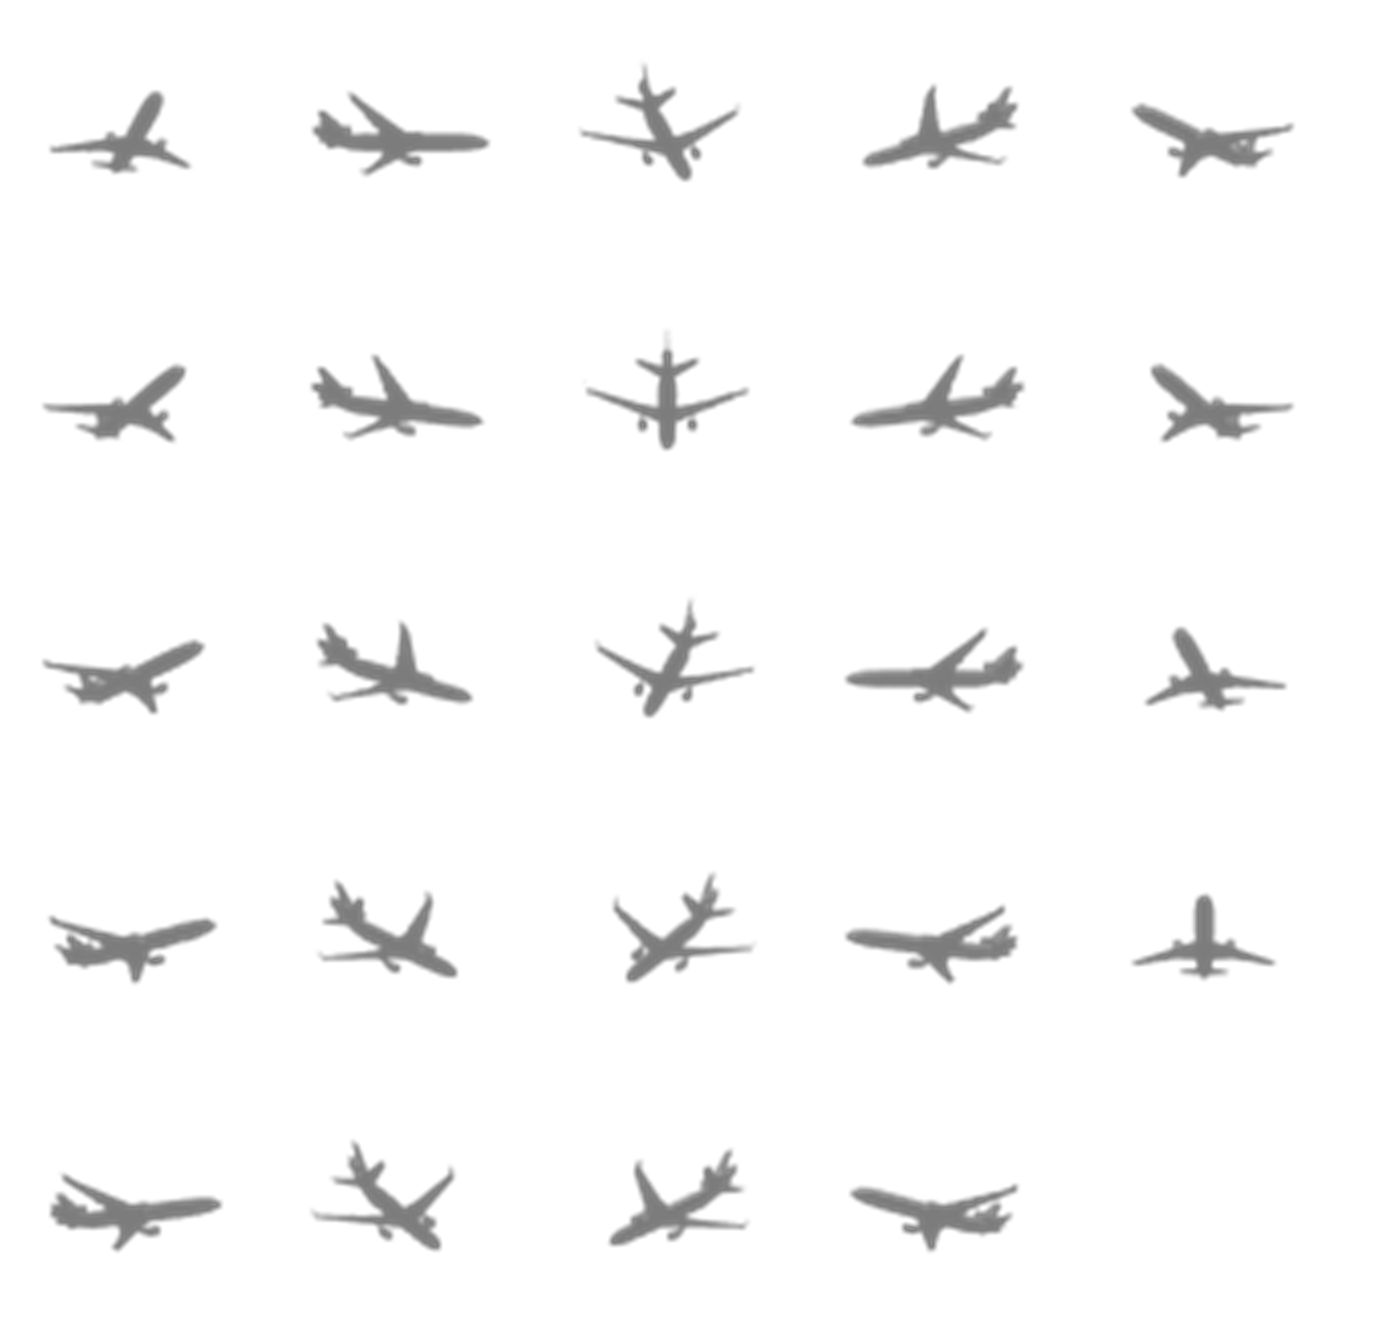
\includegraphics[width=0.5\textwidth]{images/shapenetinput.png}
  \caption{Silhouette Input from ShapeNet renders}
  \label{shapenetinput}
\end{figure}

\begin{figure}[h!]
  \centering
  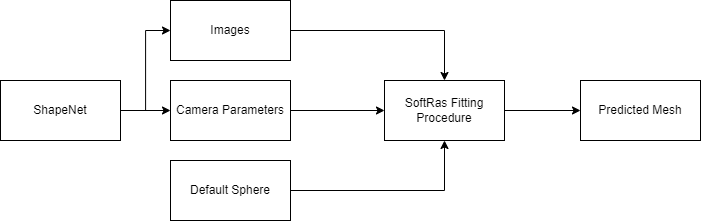
\includegraphics[width=\textwidth]{images/shapenetdatapipe.png}
  \caption{Data pipeline of original project}
  \label{shapenetdatapipe}
\end{figure}

The pipeline takes images with a 64x64 resolution, but it is extensible to other (square) resolutions. However, attempting to use much higher resolution images produces poor results, qualitatively and quantitatively, but the speed of the fitting procedure is the real limiting factor. The pipeline also takes a camera viewpoint for every image. This determines which directions the fitting procedure should generate renders of the mesh from to compute a loss between the input images and the renders.

\subsection{Algorithm Improvements}
\subsubsection{Data}
The original pipeline is built for images from ShapeNet. In order to utilise other data sources, we first build a pipeline for processing the input images. We modify SoftRas to operate on 256x256 input images. We then process input images, resizing them to this size. Details for how these images are converted to silhouettes are in \ref{section:silimp}. We also need to make adjustments to the mesh to deal with more detailed images and the details for this are in \ref{section:meshimp}. We test these changes using both ALOI, where the camera parameters and silhouettes are known, and images that we have captured, where we have no viewpoint or segmentation ground truth. Some sample images from ALOI are shown in Figure \ref{aloisamples}.

\begin{figure}[h!]
  \centering
  \begin{subfigure}{0.45\textwidth}
    \centering
    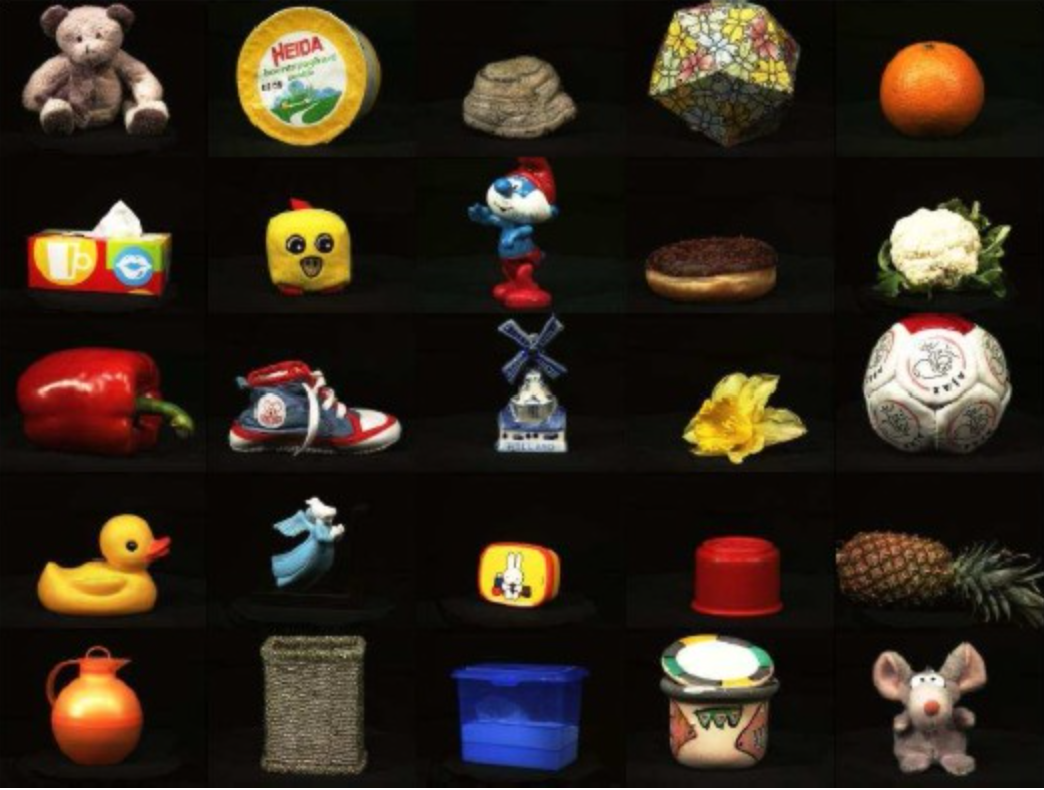
\includegraphics[width=\textwidth]{images/aloiobjects.png}
    \caption{Sample of different objects}
    \label{aloiobjects}
  \end{subfigure}
  \hfill
  \begin{subfigure}{0.45\textwidth}
    \centering
    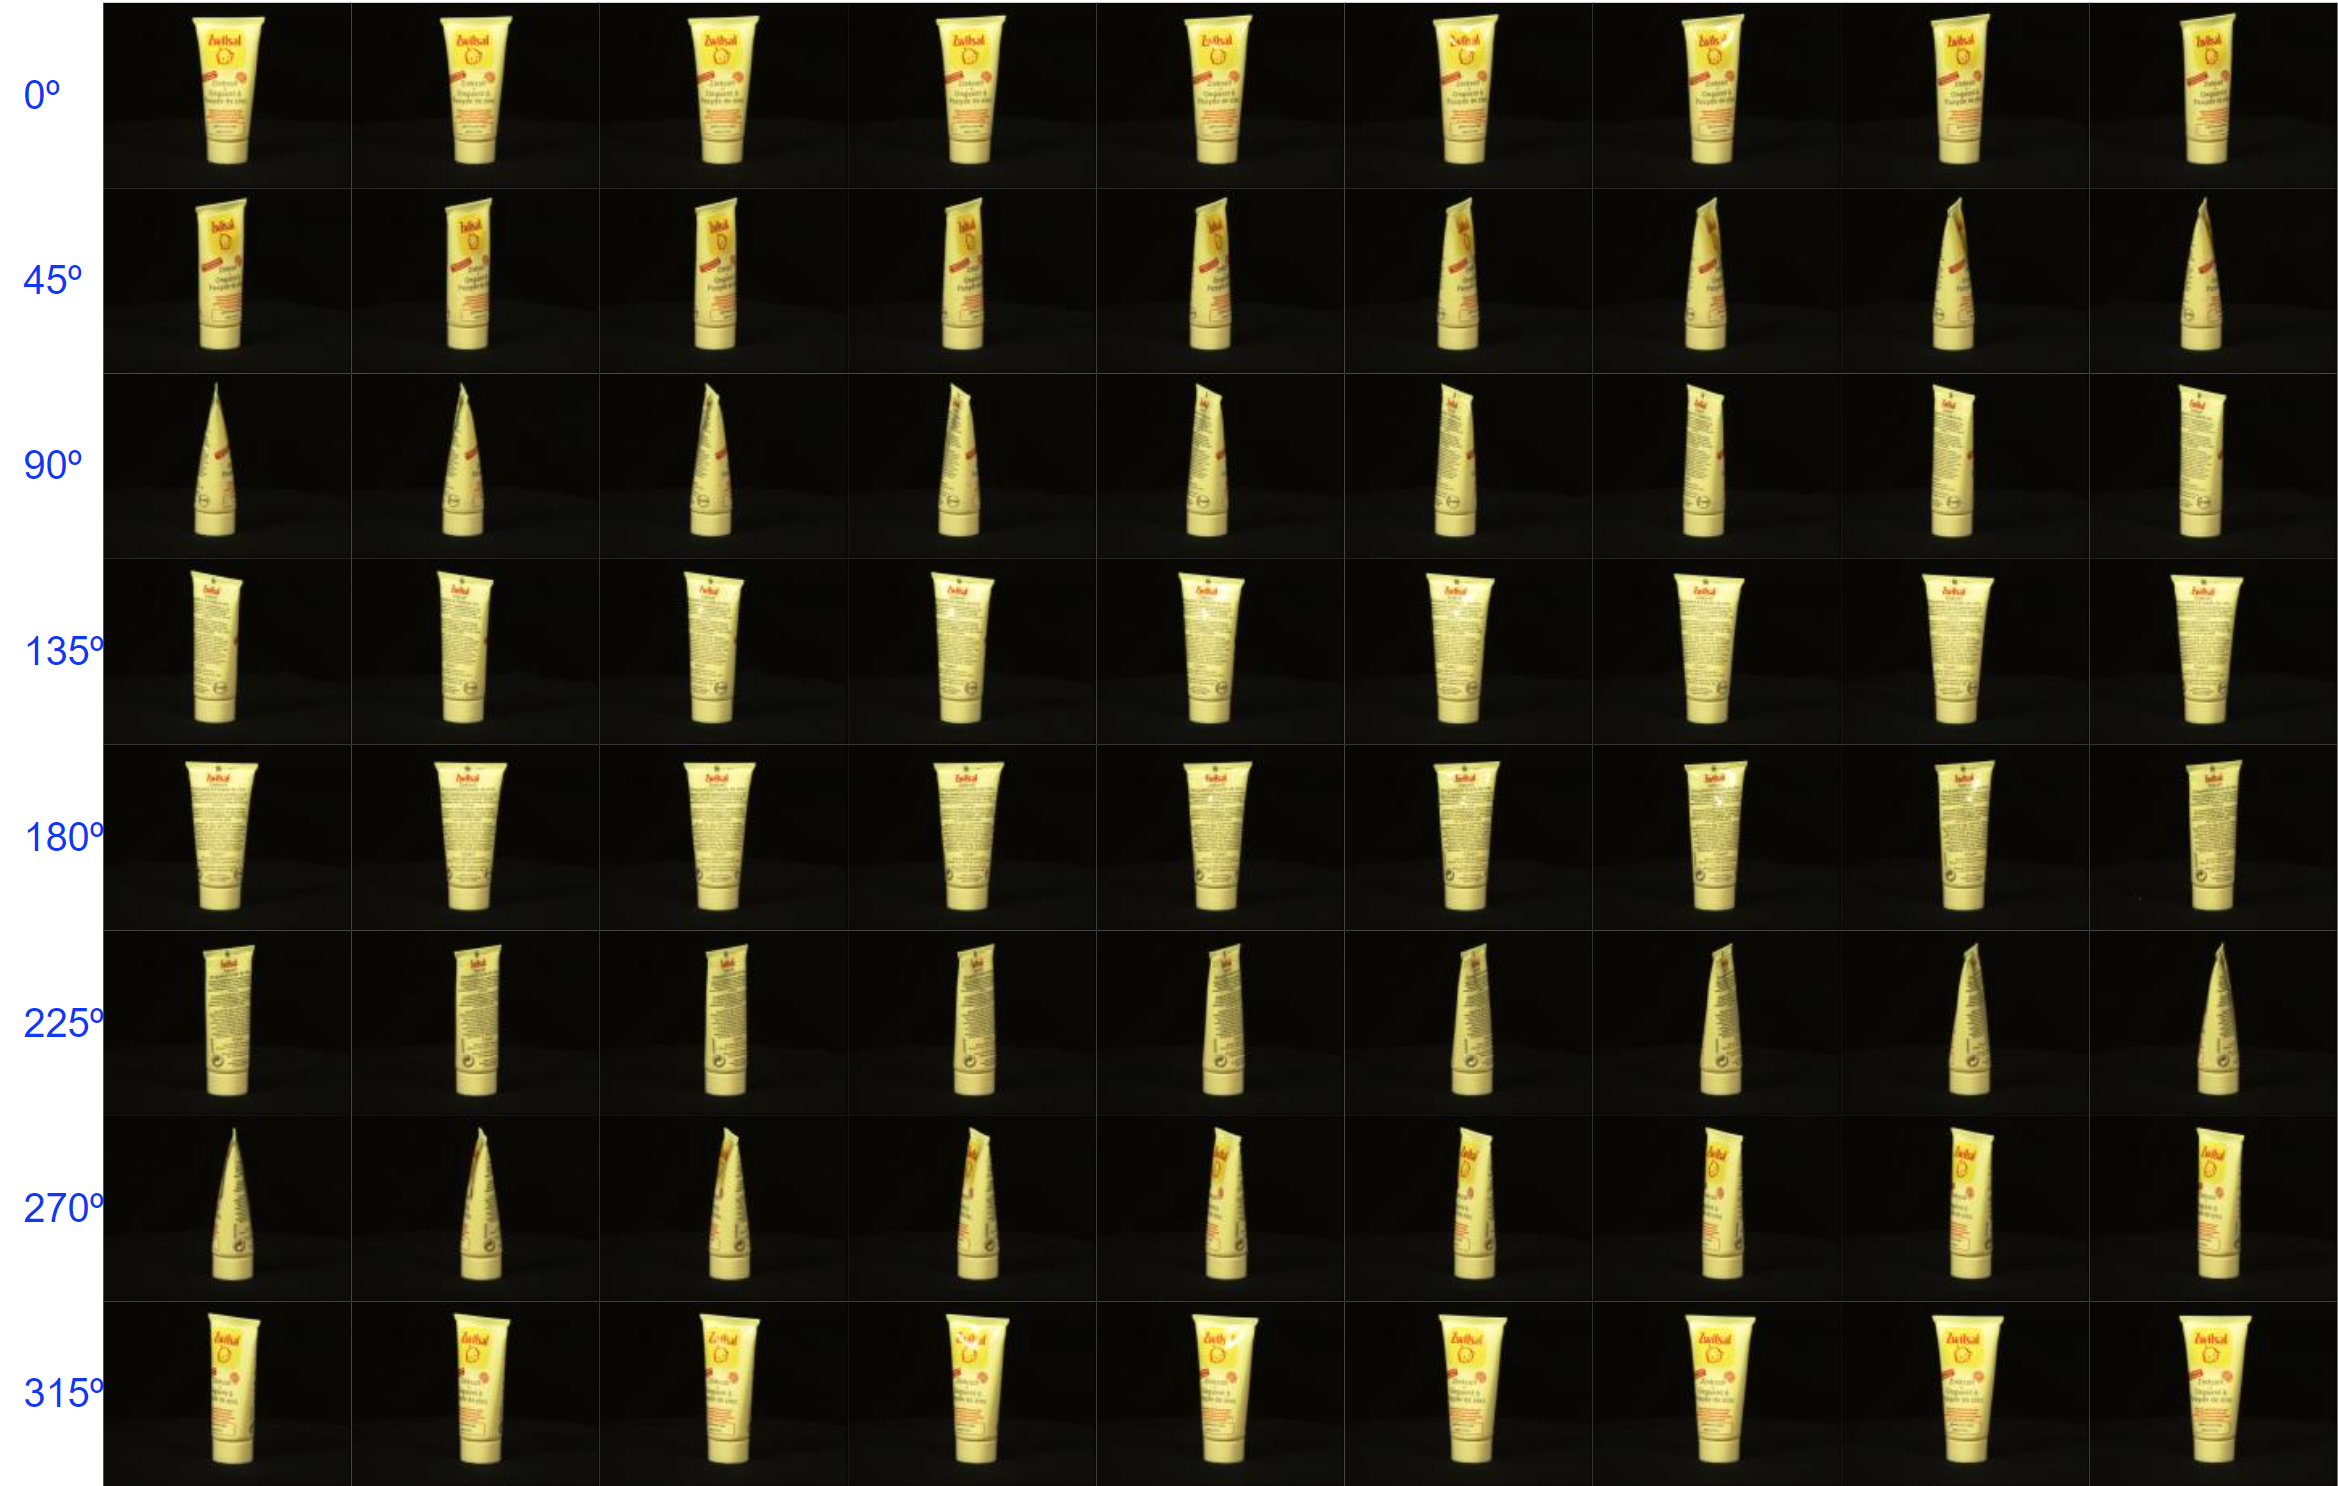
\includegraphics[width=\textwidth]{images/aloiviews.png}
    \caption{Each object is captured from 72 angles}
    \label{aloiviews}
  \end{subfigure}
  \caption{Samples from ALOI dataset.}
  \label{aloisamples}
\end{figure}

\subsubsection{Silhouette Initialisation}
\label{section:silimp}

Synthetic datasets such as ShapeNet allow us to directly produced silhouettes. For carefully produced photorealistic datasets such as ALOI, where object/background mask labels have been provided, silhouettes can be generated as shown in \ref{section:datapipe}. However, for natural images, these silhouettes have to be estiamted.

We modify the pipeline to enable fitting meshes for natural images with backgrounds. We utilise DeepLabv3, to produce a segmentation map of a set of inputs. We can then convert the semantic classifications into a binary pixel map, with 0 representing the background and 1 representing the subject of the image. We utilise this binary pixel map as the alpha channel of the image and also to set the pixel values of the background of the image to 0. We also convert the active pixel values to grey pixels, as the colour information is not utilised. These new images can be used as silhouette inputs to the standard SoftRas pipeline.

\noindent$
  I = 
  \begin{bmatrix}
    I_R & I_G & I_B\\
  \end{bmatrix}
$, where $I_R, I_G, I_B$ are matrices with values for each pixel in image $I$.

\noindent$deeplab(i) = C$, where $C$ is a matrix of semantic classifications for each pixel.

\noindent$M = (C > 0)$, where $M$ is a matrix of binary classifications (object or background) for each pixel.

\noindent$\alpha = M \times 255$, where $\alpha$ is a matrix of alpha channel values.

\noindent$I'_{i,j} = I_{i,j} * (M_{i,j} \times 124)$, where $I'$ is a greyscale version of $I$ with zeroed background pixels.

\noindent$
  I_{out} =  
  \begin{bmatrix}
    I'_R & I'_G & I'_B & \alpha\\
  \end{bmatrix}
$

\subsubsection{Mesh Initialisation}
\label{section:meshimp}
We modify the initial mesh passed to the fitting procedure. The sphere used in the original pipeline, shown in Figure \ref{sphereinit}, has some key issues.

\begin{figure}[h!]
  \centering
  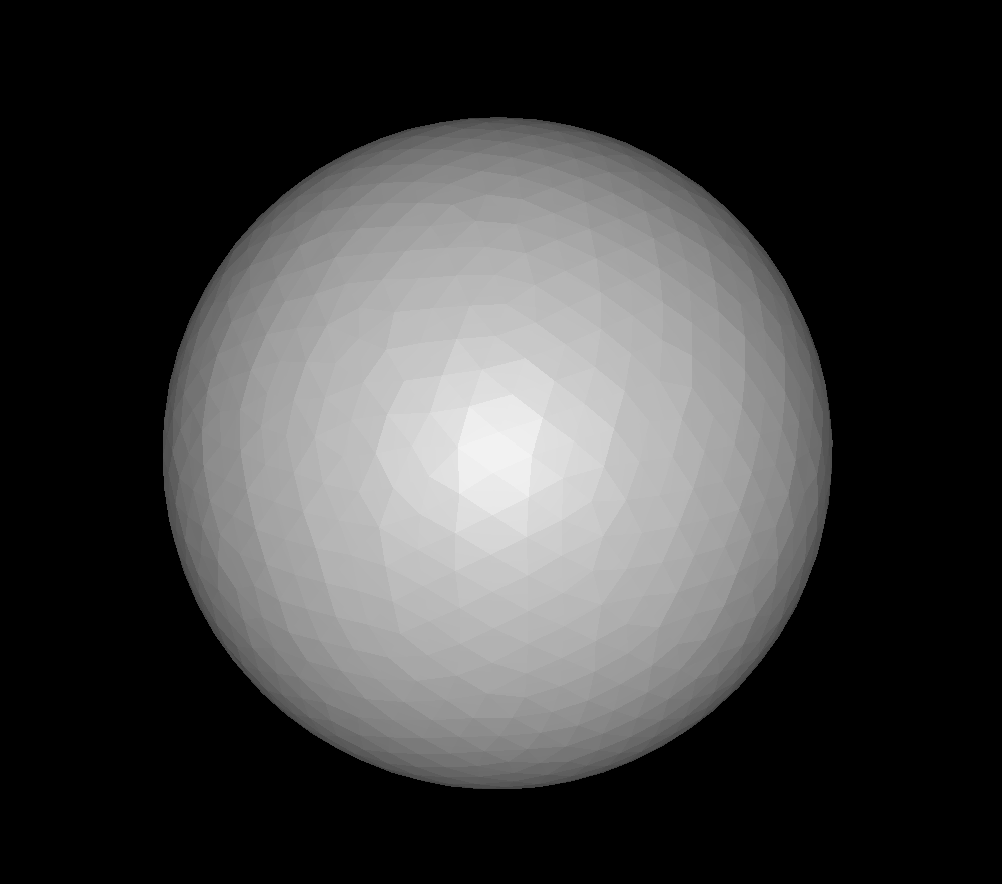
\includegraphics[width=0.35\textwidth]{images/sphereinit.png}
  \caption{Sphere initialisation}
  \label{sphereinit}
\end{figure}

A fixed size sphere is used, so if the images provided detail a subject that is much larger or smaller than the sphere, then many iterations are used to adjust the size of the mesh, if it succeeds at all. Figure \ref{apricottarget} shows an example where the position and scale of the target (a small apricot at the bottom of the image) leads to failure with the sphere initialisation. To address this, we vary the size of the initial mesh based on the input images as well as scaling the $x$ and $y$ dimensions to match the aspect ration of the target object. We do this by forming a bounding box around the target object and calculating the scale factor to modify the height and width of the sphere by accordingly. The equation below hides the complexity of converting between pixel based widths for the target image and real-world measurement units for the sphere.

\[w_{scale} = \frac{w_{sphere}}{w_{target}}\]
\[h_{scale} = \frac{h_{sphere}}{h_{target}}\]

\begin{figure}[h!]
  \centering
  \begin{subfigure}{0.25\textwidth}
    \centering
    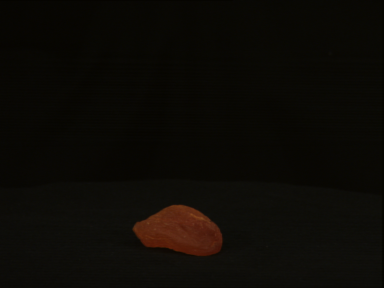
\includegraphics[width=\textwidth]{images/apricot.png}
    \caption{Target object}
    \label{apricot}
  \end{subfigure}
  \hfill
  \begin{subfigure}{0.25\textwidth}
    \centering
    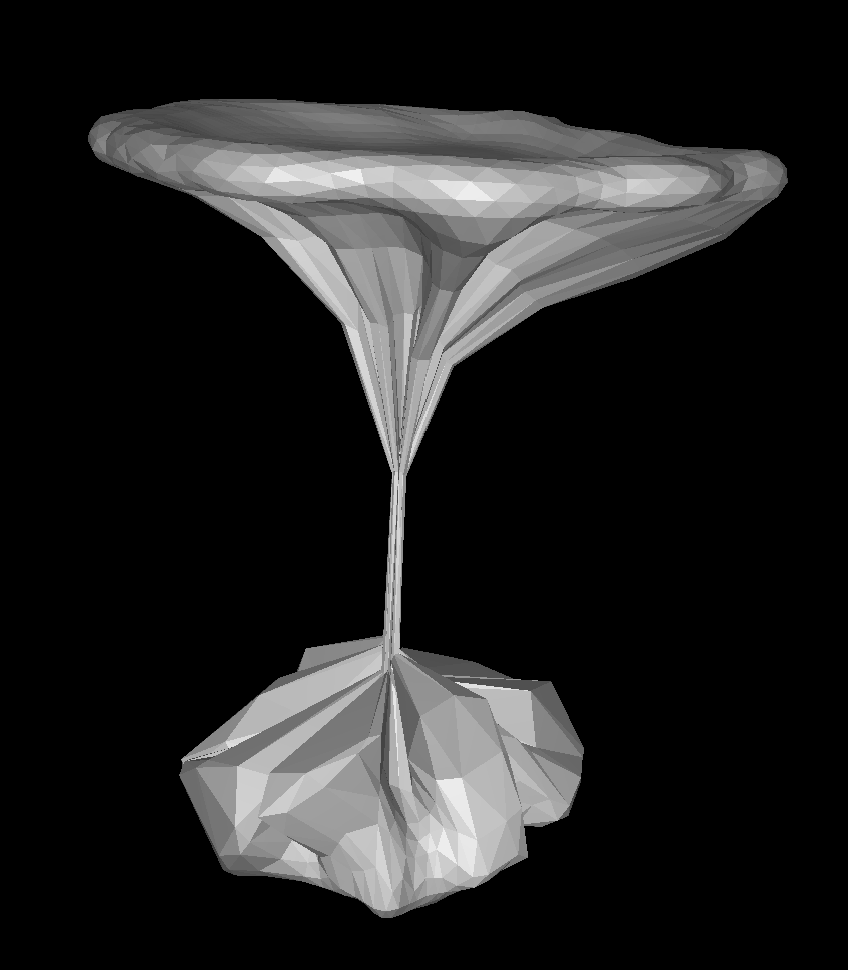
\includegraphics[width=\textwidth]{images/apricotfailure.png}
    \caption{Failure to converge}
    \label{apricotfailure}
  \end{subfigure}
  \caption{Failure to converge with sphere initialisation}
  \label{apricottarget}
\end{figure}

Another issue is that the sphere is always centred at the origin. This is not a large issue for synthetic datasets like SoftRas, but for photorealistic datasets such as ALOI or even natural images captured by a smartphone, the subject is unlikely to be centred at the origin. This means that the fitting procedure will utilise many iterations to move the mesh to where the subject is within the image. Additionally, this is actually achieved by moving individual vertices, which leads to stretching, distortion and twisting artefacts as shown in Figure \ref{buckettarget}. To address this, we translate the initial mesh according to the position of the subject within the input images. We once again achieve this using a bounding box on the target object. This step is performed after the scaling, so aligning the top and left of the sphere with the top and left of the target object is sufficient for aligning the image and mesh.

\[w_{shift} = l_{mesh} - l_{object}\]
\[h_{shift} = t_{mesh} - t_{object}\]

\begin{figure}[h!]
  \centering
  \begin{subfigure}{0.25\textwidth}
    \centering
      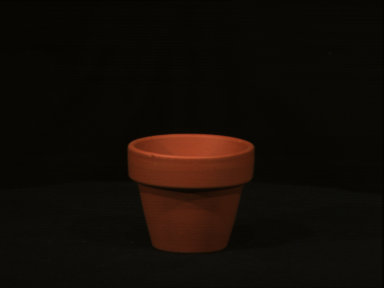
\includegraphics[width=\textwidth]{images/bucket.png}
      \caption{Target object: bucket}
      \label{bucket}
  \end{subfigure}
  \hfill
  \begin{subfigure}{0.25\textwidth}
    \centering
      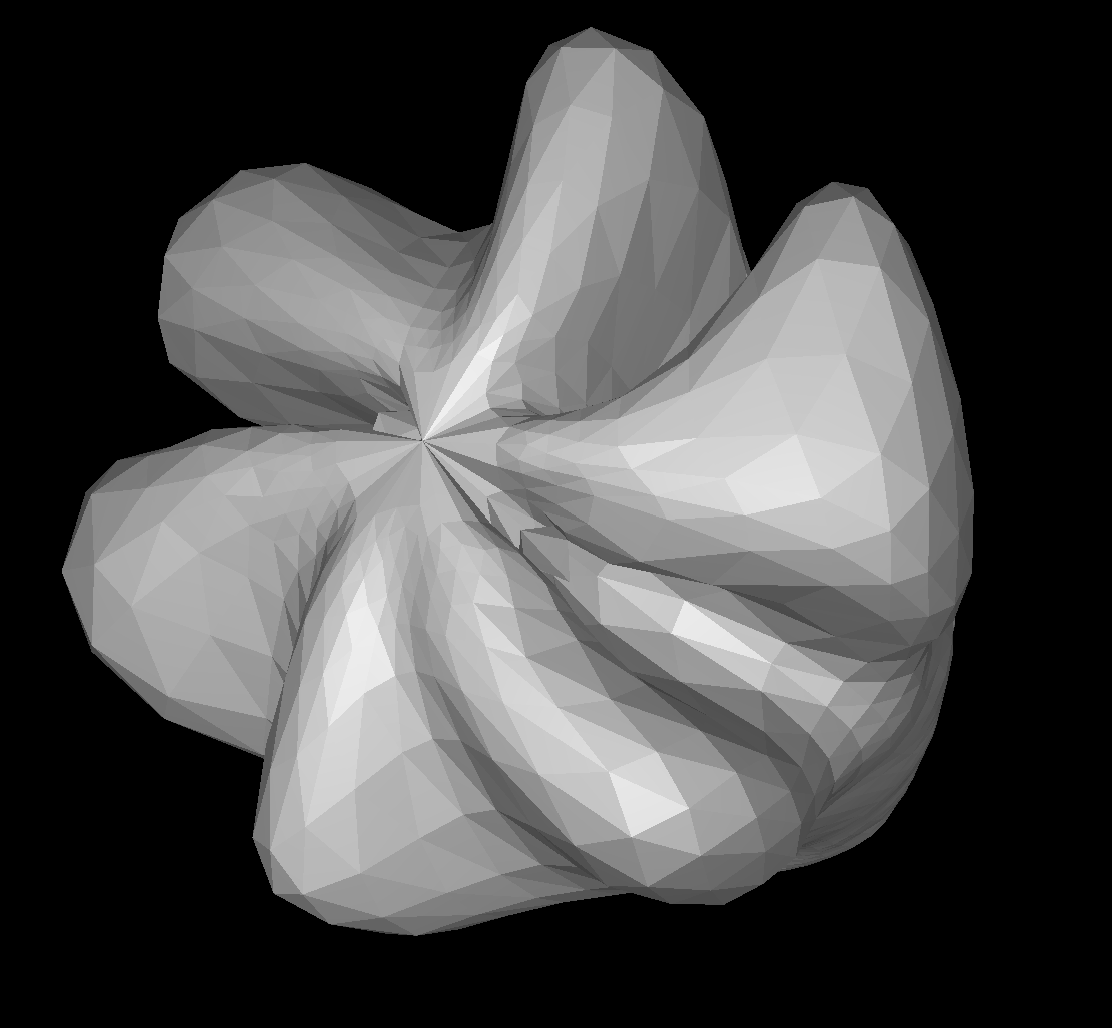
\includegraphics[width=\textwidth]{images/bucketartefact.png}
      \caption{Twisting artefacts due to off-centre target}
      \label{bucketfailure}
  \end{subfigure}
  \caption{Artefacts with sphere initialisation}
  \label{buckettarget}
\end{figure}

The sphere used in the original pipeline has roughly 1300 polygons. This polygon count does not vary during the fitting procedure, only the positions of the vertices. This is sufficient for the simple 64x64 images used in the original pipeline, but not for higher resolution images with more high frequency information. In Figure , the detail in the predicted mesh of the target is limited by the polygon count of the sphere. To address this, we replace the original initialisation sphere with a new sphere with around 1900 polygons that we created in Blender and dynamically choose the initial sphere based on the target image.

\begin{figure}[h!]
  \centering
  \begin{subfigure}{0.25\textwidth}
    \centering
    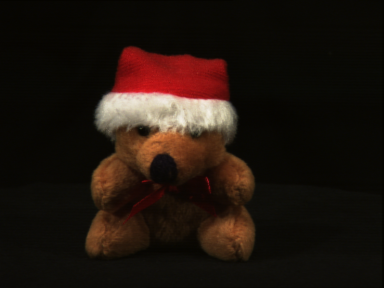
\includegraphics[width=\textwidth]{images/teddy.png}
    \caption{Target object}
    \label{teddy}
  \end{subfigure}
  \hfill
  \begin{subfigure}{0.25\textwidth}
    \centering
    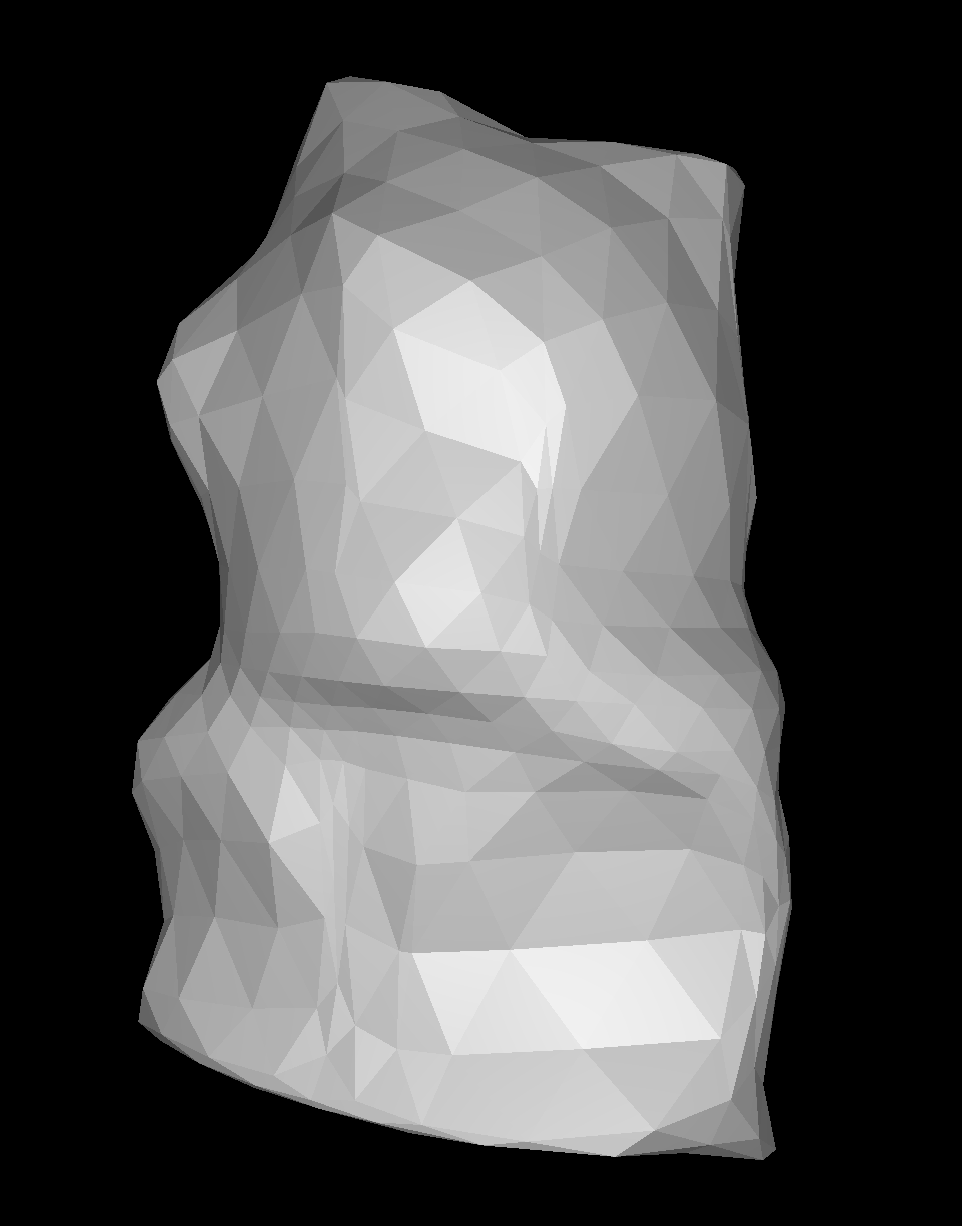
\includegraphics[width=\textwidth]{images/teddyfailure.png}
    \caption{Lack of detail in reconstruction}
    \label{teddyfailure}
  \end{subfigure}
  \caption{Lack of detail when attempting to fit to larger targets with many folds}
  \label{teddytarget}
\end{figure}

\subsection{Implementation Details}

\subsubsection{Data Pipeline}
\label{section:datapipe}

The original dataset uses images and viewpoint parameters from ShapeNet stored as NumPy array files as inputs. To make the pipeline extensible, this is replaced with a folder input for images. The camera parameters can then be given according to the ground truth of the dataset or inferred from the images. This enables us to switch between data sources and image samples by simply editing the image source path. All input images are resized to 256x256 as this was found to be a sweetspot for execution time for the fitting procedure.

The ALOI dataset images are taken every 5 degrees in a complete rotation around the object. The camera parameters can be inferred from this information. The code used to perform this initialisation is shown in Figure \ref{camerainitaloi}.

\begin{figure}[h!]
  \centering
  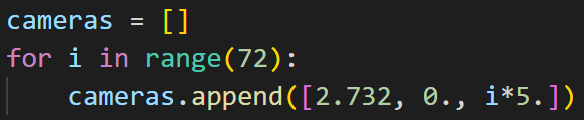
\includegraphics[width=0.35\textwidth]{images/initcamera.png}
  \caption{Viewpoint parameter initialisation for ALOI}
  \label{camerainitaloi}
\end{figure}

The ALOI dataset also comes with ground truth object/background binary masks, which we utilise to generate silhouettes from the raw images. This is shown in Figure \ref{datapipeline}. We experimented with greyscale and colour silhouettes and found no difference in results (as colour is not considered in the loss computation), so we converted the silhouettes to grey scale.

\begin{figure}[h!]
  \centering
  \begin{subfigure}{0.23\textwidth}
    \centering
    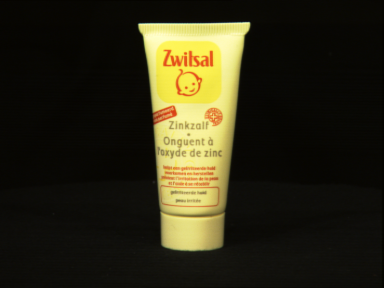
\includegraphics[width=\textwidth]{images/moisturiserpng.png}
    \caption{Original image (384 x 288)}
    \label{moistpng}
  \end{subfigure}
  \hfill
  \begin{subfigure}{0.23\textwidth}
    \centering
    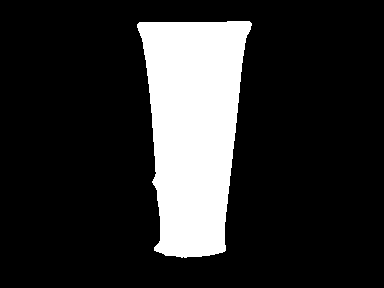
\includegraphics[width=\textwidth]{images/moisturisermask.png}
    \caption{Ground truth mask (384 x 288)}
    \label{moistmask}
  \end{subfigure}
  \hfill
  \begin{subfigure}{0.23\textwidth}
    \centering
    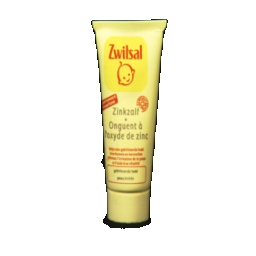
\includegraphics[width=\textwidth]{images/moisturisersil.png}
    \caption{Generated silhouette (256x256)}
    \label{moistsil}
  \end{subfigure}
  \hfill
  \begin{subfigure}{0.23\textwidth}
    \centering
    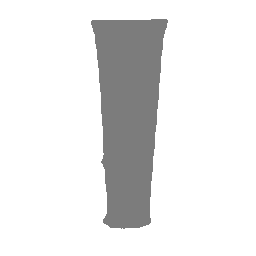
\includegraphics[width=\textwidth]{images/moisturisersilgrey.png}
    \caption{Generated silhouette greyscale (256x256)}
    \label{moistsilgrey}
  \end{subfigure}
  \caption{Image pipeline for ALOI}
  \label{datapipeline}
\end{figure}

\subsubsection{Silhouette Initialisation}

As stated in \ref{section:silimp}, we estimate silhouettes for natural images using segmentation. This is performed in the segment.py module as shown in Figure \ref{segment}. 

\begin{figure}[h!]
  \centering
  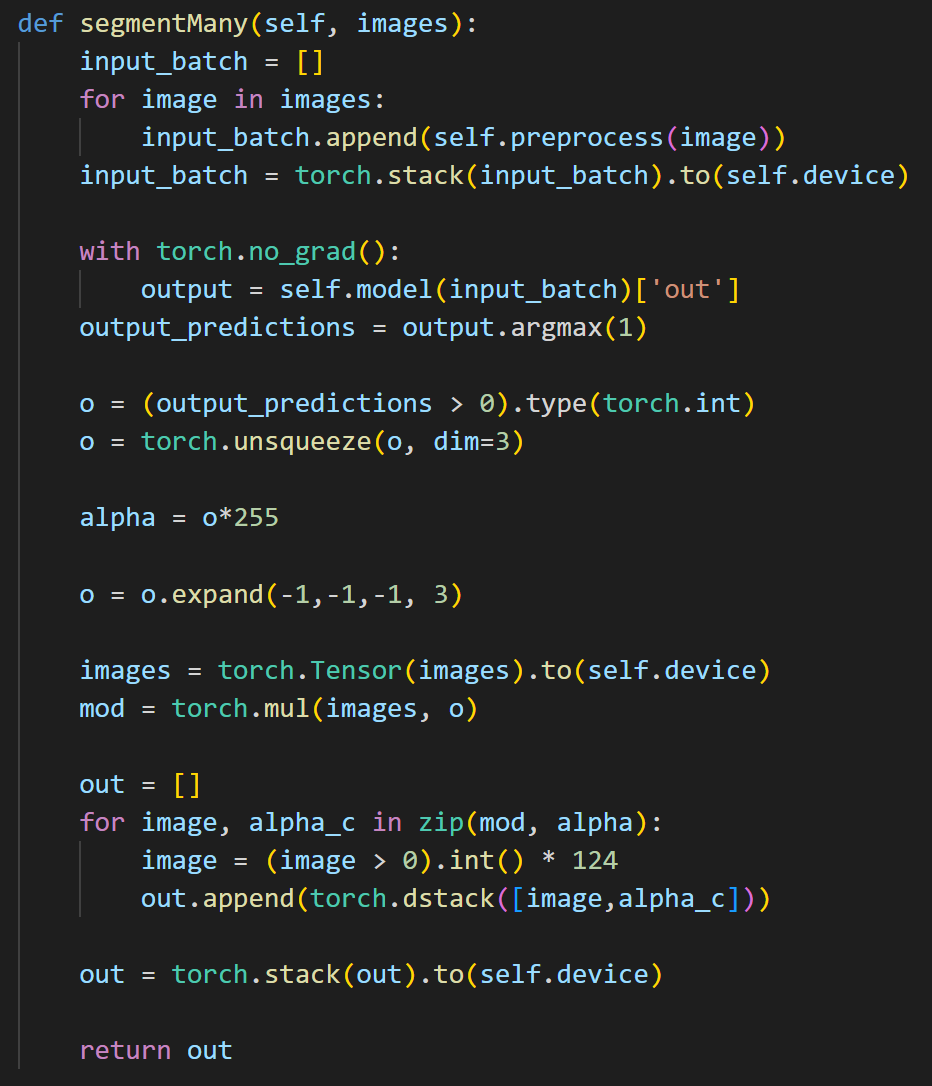
\includegraphics[width=0.5\textwidth]{images/segmentcode.png}
  \caption{Code used to perform segmentation using DeepLabv3}
  \label{segment}
\end{figure}

\subsubsection{Mesh Initialisation}

We create higher polygon count sphere initialisations in Blender using a simple UV sphere and the subdivide functionality. The straightforward process is shown if Figure \ref{blender}. We also modify the SoftRas pipeline to deal with 256x256 images, which is a simple parameter change when initialsing the soft rasteriser during the fitting procedure.

\begin{figure}[h!]
  \centering
  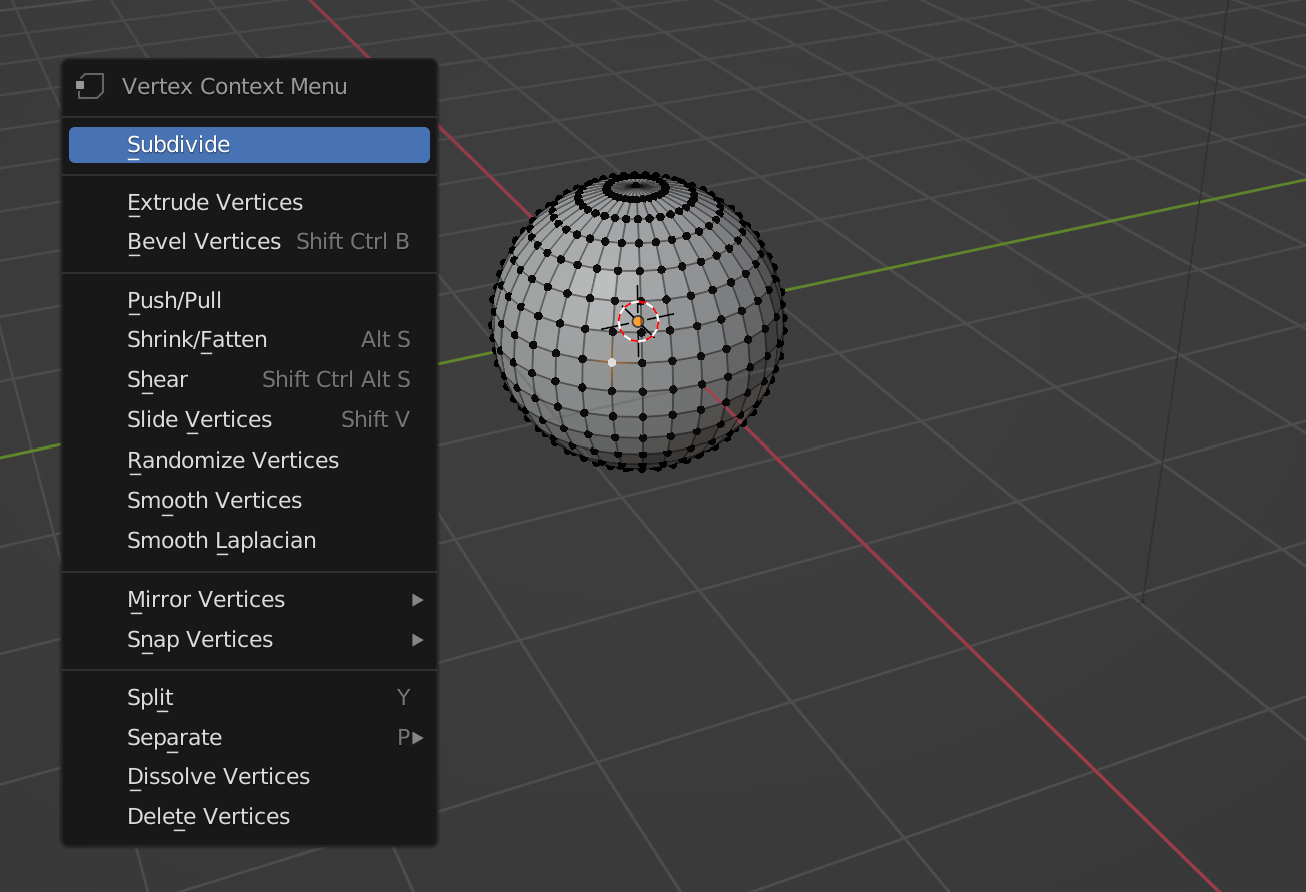
\includegraphics[width=0.5\textwidth]{images/blender.png}
  \caption{Creating higher polygon count spheres in Blender}
  \label{blender}
\end{figure}

In order to modify this mesh according to the target object, we first examine an image of the target object as shown in Figure \ref{imageeval}. This gives us the height and width of the object in pixels, as well as the top and left of the object in terms of the image dimensions.

\begin{figure}[h!]
  \centering
  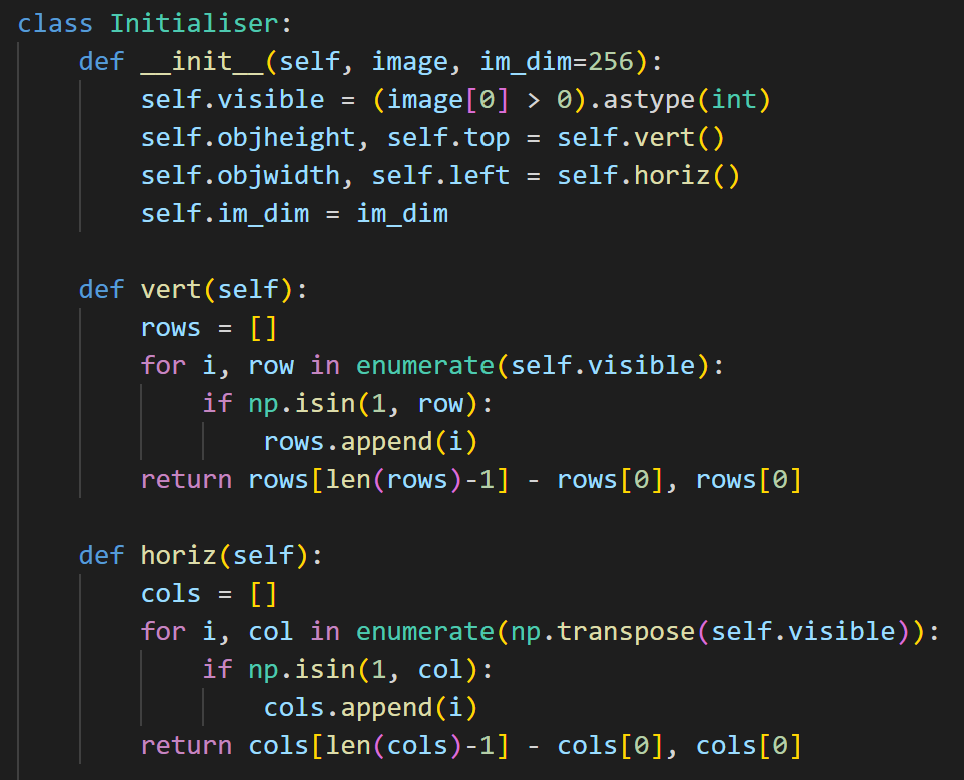
\includegraphics[width=0.5\textwidth]{images/image_eval.png}
  \caption{Inferring information about the target object from a target image}
  \label{imageeval}
\end{figure}

The first step is to scale the $x$ and $y$ dimensions of the sphere according the the aspect ratio and size of the target object. The code for this is shown in Figure \ref{scalecode}.

\begin{figure}[h!]
  \centering
  \begin{subfigure}{0.4\textwidth}
    \centering
    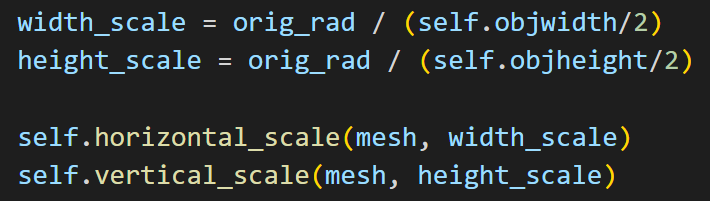
\includegraphics[width=\textwidth]{images/scale_a.png}
    \caption{Calculate the scale factors}
  \end{subfigure}
  \hfill
  \begin{subfigure}{0.4\textwidth}
    \centering
    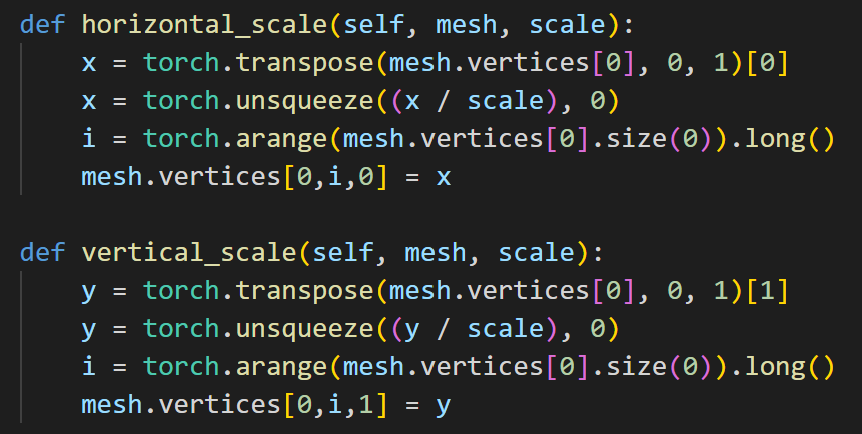
\includegraphics[width=\textwidth]{images/scale_b.png}
    \caption{Scale the mesh accordingly}
  \end{subfigure}
  \caption{Scaling the initial mesh according to the target object}
  \label{scalecode}
\end{figure}

We can then shift the initial mesh according to where in the 256x256 image the target object is. The code for this is shown in Figure \ref{shiftcode}.

\begin{figure}[h!]
  \centering
  \begin{subfigure}{0.4\textwidth}
    \centering
    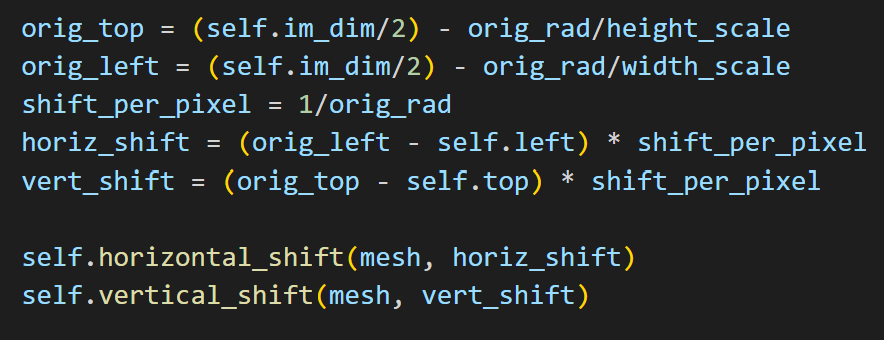
\includegraphics[width=\textwidth]{images/shift_a.png}
    \caption{Calculate the shift amounts}
  \end{subfigure}
  \hfill
  \begin{subfigure}{0.4\textwidth}
    \centering
    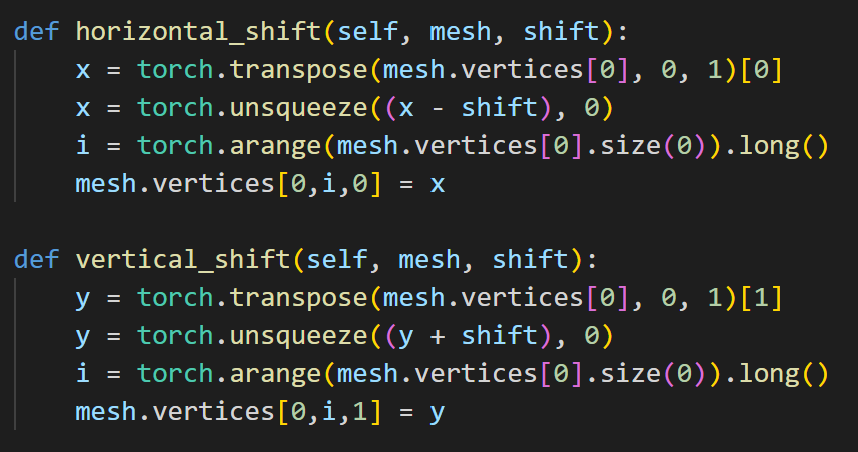
\includegraphics[width=\textwidth]{images/shift_b.png}
    \caption{Shift the mesh accordingly}
  \end{subfigure}
  \caption{Translating the initial mesh according to the target object}
  \label{shiftcode}
\end{figure}

\subsection{Data Pipelines}

Figure \ref {aloidatapipe} shows the new data pipeline for testing using the ALOI dataset.

\begin{figure}[h!]
  \centering
  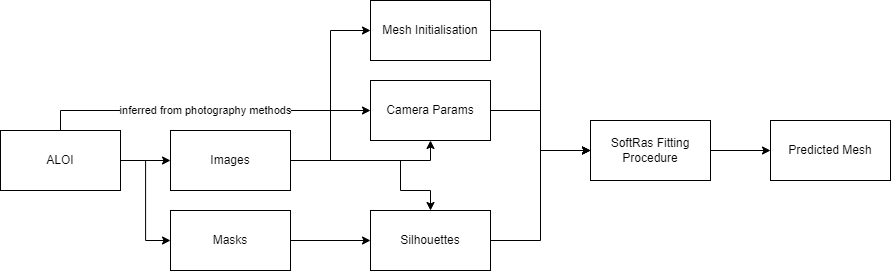
\includegraphics[width=\textwidth]{images/aloidatapipe.png}
  \caption{Data pipeline using ALOI dataset}
  \label{aloidatapipe}
\end{figure}

Figure \ref {natdatapipe} shows the data pipeline when we utilise novel images.

\begin{figure}[h!]
  \centering
  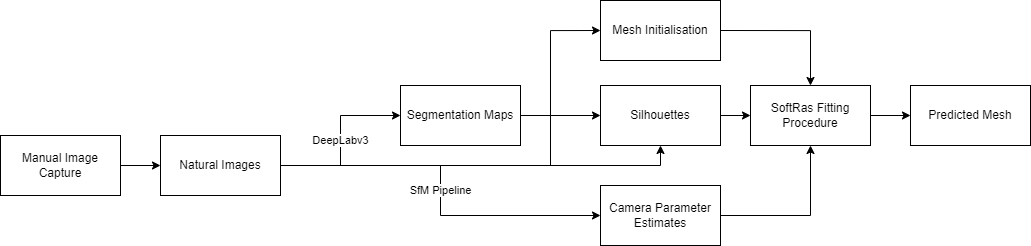
\includegraphics[width=\textwidth]{images/natdatapipeline.png}
  \caption{Data pipeline for newly captured images}
  \label{natdatapipe}
\end{figure}

\subsection{Fitting Procedure}

Modified fitting procedure from softras demo. Uses Adam optimiser.

\newpage
\section{Experiments and Evaluation}
\subsection{Datasets}

A key focus of our project is to investigate the performance of SoftRas on higher resolution, photorealistic data. For this, we utilise the Amsterdam Library of Objects (ALOI) dataset \parencite{aloi}. It contains images of 1000 small objects at a resolution of 384 x 288. Shown below are some samples from the dataset.

COMPARE SHAPENET AND ALOI RESULTS

\subsubsection{Quantitive}
\subsubsection{Qualitative}

\subsection{Silhouette Initialisation}

COMPARE SEGMENTED IMAGES WITH MASKS

\subsubsection{Quantitive}
\subsubsection{Qualitative}

\subsection{Mesh Initialisation}

COMPARE DIFFERENT INITIALISATIONS

\subsubsection{Quantitive}
\subsubsection{Qualitative}

\subsection{Camera Initialisation}
\subsubsection{Quantitive}
\subsubsection{Qualitative}

\newpage
\section{Conclusions and Future Directions}
\subsection{Conclusions}
\subsection{Discussion of Limitations}
\subsection{Future Directions}
\newpage
\printbibliography[
  heading=bibintoc,
  title={References}
]
\newpage
\section*{Appendicies}
\newpage

\end{document}